
\documentclass{article} % For LaTeX2e
\usepackage{iclr2027_conference,times}

% Optional math commands from https://github.com/goodfeli/dlbook_notation.
\input{math_commands.tex}

\usepackage{hyperref}
\usepackage{url}
\usepackage{amsmath}
\usepackage{amssymb}
\usepackage{multirow}
\usepackage{amsthm}
\usepackage{booktabs}
\usepackage{float}
\usepackage{placeins}
\usepackage{enumitem}
\usepackage{graphicx}
\usepackage{tikz}
\usepackage{xcolor}
% --- bulleted paragraph bodies -----------------------------------------
\newenvironment{pb}{\begin{itemize}\setlength\itemsep{2pt}%
  \setlength\parskip{0pt}\setlength\topsep{2pt}\setlength\partopsep{0pt}}%
  {\end{itemize}}

\usetikzlibrary{positioning,fit,backgrounds,arrows.meta,calc,shapes.geometric}

% ---- method-figure palette ----
\definecolor{accent}{HTML}{0F8F86}
\definecolor{sone}{HTML}{3F6BD6}
\definecolor{stwo}{HTML}{9A5A2B}
\definecolor{ink}{HTML}{1B2026}
\definecolor{sonebg}{HTML}{E8EEFB}
\definecolor{stwobg}{HTML}{F6EDE1}
\definecolor{accbg}{HTML}{E2F4F1}
\definecolor{greyb}{HTML}{F1F3F6}
\definecolor{store}{HTML}{4A5360}
\definecolor{dltgreen}{HTML}{1F7A4A}
% tab:stage2swap 的增量下标:比正常下标再小一档;均值列那一格用绿色
\newcommand{\dlt}[1]{$_{\scriptscriptstyle#1}$}
\newcommand{\dltg}[1]{$_{\scriptscriptstyle\textcolor{dltgreen}{#1}}$}

% ---- theorem environments (appendix theory) ----
\newtheorem{proposition}{Proposition}
\newtheorem{corollary}{Corollary}
\newtheorem{remark}{Remark}
\newcommand{\Mten}{\mathrm{M}}

% ======================================================================
% DRAFT v1 (2026-08-14). Skeleton / bullet outline, not committed prose.
% Framing: "An Effective / Practical Way to X" (breadth + robustness,
% not single-point SOTA); ICLR-leaning intro (discrimination is already
% in frozen features; aggregation can be READ, not learned).
% Table 1 numbers are PEAK backbone/operator per set = upper bound.
% [TODO] = load-bearing pending work.
% ======================================================================

\title{Patches Are Enough: Simple and Effective \\ Training-Free Visual Place Recognition}

\author{Anonymous authors \\ Paper under double-blind review}

%\iclrfinalcopy % Uncomment for camera-ready version, but NOT for submission.
% 浮动体参数放宽:表多且大,默认参数会把浮动体推到文末
\renewcommand{\topfraction}{0.95}
\renewcommand{\bottomfraction}{0.9}
\renewcommand{\textfraction}{0.05}
\renewcommand{\floatpagefraction}{0.8}
\setcounter{topnumber}{3}
\setcounter{totalnumber}{5}

\begin{document}

\maketitle

\begin{abstract}
Visual Place Recognition (VPR) asks where a photograph was taken by retrieving the most similar image from a geo-tagged database. Training a representation for it calls for a place-labelled corpus running to tens of millions of images, produces features that shift with the domain, and ties the result to the one backbone it was trained on. Methods built on frozen foundation models avoid all three and need no place label, yet they still trail supervised ones. They choose what to keep from an image by salience, which is not the property that separates places. In this paper we remove that criterion and let the patches of the two images being compared supply every quantity in the pipeline. Two tables of patch-to-patch similarity carry it: the self-similarity of one image weights each patch by how many of that image's own patches resemble it, in closed form; the cross-similarity of the pair is reduced two ways, one factoring into a per-image covariance that scans a database, the other not factoring and re-ranking a shortlist. Nothing is fitted between the frozen network and the ranking. Across thirteen benchmarks spanning urban streets, seasonal railways, and degraded, subterranean, indoor, aerial and underwater imagery, one fixed configuration reaches the highest mean Recall@1, and it is level with the strongest supervised method on the urban benchmarks its supervision targets. As a drop-in scoring rule, it also improves published two-stage pipelines when it replaces their own re-ranker and single-stage ones when it is added to them.
\end{abstract}

\section{Introduction}
\begin{figure}[htbp]
\centering
\makebox[\linewidth][c]{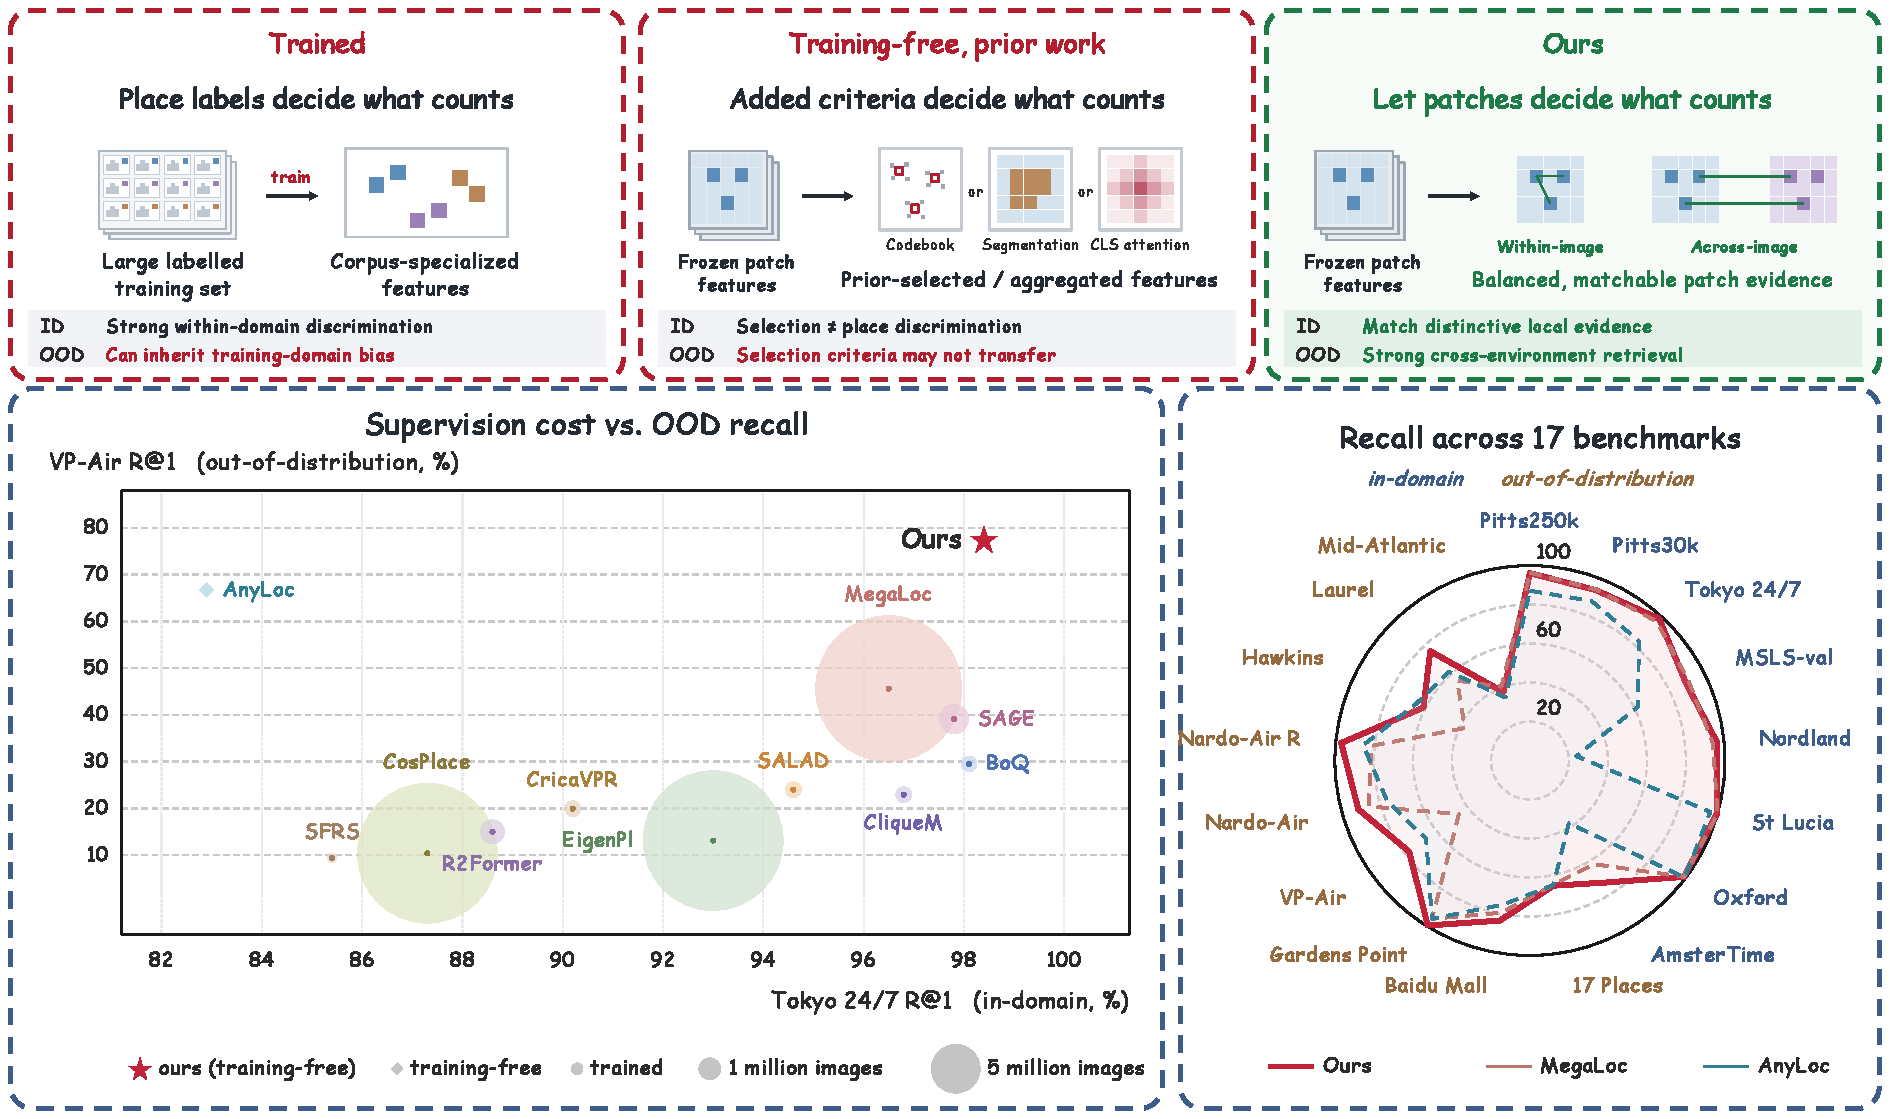
\includegraphics[width=\linewidth]{figures/teaser_v6.pdf}}
% \caption{\textbf{Three ways of deciding what an image contributes.} \textbf{A}: a representation shaped by place-labelled supervision. \textbf{B}: patches selected or aggregated by a criterion fixed outside the pair of images. \textbf{C}: ours, where both decisions are read from patch-to-patch similarities inside the pair. \textbf{D}: mean R@1 on the 8 standard benchmarks against the 9 cross-environment ones, with marker size increasing with the number of labelled training images; SFRS is omitted, its standard mean falling far below the range shown. \textbf{E}: R@1 on all 17 benchmarks.
\caption{\textcolor{red}{\textbf{Overview and performance (R@1).} (A) Trained methods require large-scale labelled datasets, limiting their generalisation to cross-environment settings. (B) Prior training-free methods avoid this training cost and generalise better, but suffer a performance drop on standard VPR benchmarks. (C) Our training-free method instead applies frozen patch features directly, using patch similarity both within and across images for retrieval. (D) Training cost versus performance of our method and baselines on 17 benchmarks, averaged separately across standard and cross-environment VPR benchmarks. (E) Performance of the proposed method against the state-of-the-art trained and training-free baselines.}}
\label{fig:teaser}
\end{figure}
% Visual Place Recognition (VPR), also known as visual geo-localization, is a fundamental task in computer vision that aims to determine where a photograph was taken by matching it against a database of geo-tagged images. It underpins loop closure in visual SLAM, re-localization for autonomous driving where satellite positioning is unreliable, and city-scale mapping services that anchor imagery to a map, and increasingly it is asked to work where no street-view corpus exists: aerial and drone navigation, inspection robots in mines, caves and tunnels, indoor delivery and service robots, underwater vehicles surveying the sea floor, and the matching of historical photographs to the present day. The databases involved range from a few hundred images in an indoor survey to tens of millions across a city, so a practical system has to stay accurate as the imagery, the environment and the scale of the map change.

Visual Place Recognition (VPR) is a long-standing computer vision challenge that aims to recognise where a query image was captured by matching it to a database of images tagged with their locations. VPR is essential to many core applications, such as visual SLAM, re-localisation in autonomous driving, and city-scale mapping services. Classical and standard VPR benchmarks mainly target this setting, using largely standard street-view images. However, we notice that VPR is increasingly required in a broader range of scenarios~\citep{anyloc}, such as aerial and drone navigation, indoor delivery and service robots, underwater vehicles surveying the sea floor, and the matching of historical photographs to present-day scenes. We refer to these scenarios and their corresponding benchmarks as cross-environment benchmarks. In this paper, we argue that advanced VPR solutions should generalise not only to standard VPR benchmarks but also to cross-environment benchmarks.

% Existing approaches fall into two families. The dominant family learns a representation from place labels. NetVLAD \citep{netvlad} makes soft assignment to a codebook differentiable and trains it under weak supervision, and later work follows this template through classification over geographic cells \citep{cosplace,eigenplaces}, curated labels at scale \citep{gsvcities}, feed-forward pooling \citep{mixvpr}, and aggregation over frozen DINOv2 \citep{dinov2} tokens with optimal transport \citep{salad}, learned queries \citep{boq} or adapters \citep{selavpr}. The accuracy of these methods is bought with annotation: GSV-Cities \citep{gsvcities} provides about half a million street-level images over sixty thousand labelled places, the SF-XL line \citep{cosplace,eigenplaces} trains on more than forty million, and recent systems combine several such corpora or tune the backbone itself under parameter-efficient schemes \citep{megaloc,sage}. The second family removes the annotation and reads a frozen foundation model directly, aggregating patch tokens against a fitted vocabulary \citep{anyloc}, over segmentation proposals \citep{segvlad}, or at keypoints selected by class-token attention \citep{effovpr}.

Existing VPR methods are mainly training-based approaches, which require a large amount of annotated data for training. Classical methods such as NetVLAD~\citep{netvlad} make soft assignment to a codebook differentiable and train it under weak supervision, while later work follows this template through classification over geographic cells~\citep{cosplace,eigenplaces}, curated labels at scale~\citep{gsvcities}, or feed-forward pooling~\citep{mixvpr}, among others. Recent advanced methods achieve large performance improvements, but these gains are largely driven by increasingly large-scale annotated training sets: for example, GSV-Cities~\citep{gsvcities} provides about half a million street-level images over sixty thousand labelled places, while the SF-XL dataset~\citep{cosplace,eigenplaces} contains more than forty million annotated samples. Recent state-of-the-art methods, such as~\citep{megaloc}, gather even more annotated samples to train their models, achieving the best results but relying heavily on the scale of the annotated training set, as shown in Figure~\ref{fig:teaser}D. Even with millions of annotated samples, however, these state-of-the-art methods tend to learn environment- or domain-specific features that do not generalise well as shown in Figure~\ref{fig:teaser}A), suffering a performance drop on cross-environment benchmarks, as shown in Figure~\ref{fig:teaser}D\&E. 
% Recent training-free VPR methods~\citep{anyloc} remove the large scale annotation dependency and utilize a frozen large vision model directly with some post processing which  against a fitted vocabulary \citep{anyloc}, over segmentation proposals \citep{segvlad}, or at keypoints selected by class-token attention \citep{effovpr}.


To address this data-dependency challenge, training-free VPR methods have recently been proposed~\citep{anyloc,effovpr}, which aim to exploit the generalisation ability of large vision models, such as DINO backbones~\citep{dinov2} or SAM~\citep{kirillov2023segment}, to better solve VPR across a wide range of environments. These methods often generalise better than trained methods in the cross-environment setting, but fail on standard VPR benchmarks, as shown in Figure~\ref{fig:teaser}D-E. We argue that current training-free methods, which apply various strategies to obtain prior-selected features (Figure~\ref{fig:teaser}B), do not fully utilise the potential of these large vision models.
% However, both families decide what an image contributes using information from outside the pair of images being compared, and Figure~\ref{fig:teaser} illustrates the cost. The first cell of the top row depicts the supervised recipe, in which an image is related to a labelled corpus. The learned features therefore inherit the imagery that corpus contains, and the scatter plot below makes the consequence explicit: every trained method sits high on the standard axis and low on the cross-environment one, while the marker area records the millions of labels it consumed. The second cell depicts the training-free recipe, in which a patch is related to a criterion fixed elsewhere, such as an attention map trained to locate objects in web photographs, a codebook estimated on another collection, or a segmenter's notion of an object. None of these criteria was designed to answer which parts of a scene identify a place. The two questions differ: a single window in a facade of identical windows is locally salient and is retained, yet it cannot distinguish this building from its neighbour, whereas a plain strip of pavement that appears once may be the only distinctive content in the frame. On street-view imagery the two answers coincide often enough that the substitution is harmless. Away from street view they diverge, and the training-free method that selects patches by attention loses $11.6$ mean R@1 between the two blocks (Table~\ref{tab:breadth}). This is why training-free methods, despite requiring no data, still trail supervised ones in accuracy.

% To address these issues, we propose \method{}, a training-free VPR pipeline that keeps the decision inside the pair of images being compared, as shown in the third cell of Figure~\ref{fig:teaser}. \method{} reads two tables of patch similarity from a single frozen forward pass. Within an image, its self-similarity is thresholded and summed along each row, which counts how many of the image's own patches resemble a given one; the reciprocal of this count is the distinctiveness of that patch, and it solves a classical democratic-aggregation condition when repeated content forms blocks of near-duplicates. Between two images, the cross-similarity table is reduced in two ways: a bilinear contraction that factorizes into one descriptor per image and scans the database, and a row-wise maximum that does not factorize and fine-ranks a shortlist. Extensive experiments on seventeen benchmarks, under a single configuration held fixed throughout, show that \method{} achieves $93.2$ mean Recall@$1$ on eight standard VPR benchmarks and $76.6$ on nine cross-environment benchmarks spanning degraded, subterranean, indoor, aerial and underwater imagery, compared with $65.1$ for the strongest supervised method on the latter.

\textcolor{red}{To address these challenges, we propose \method{} (Unified Patch Similarity), a simple and effective training-free method for VPR. \method{} first partitions the input images, whether queries or database images, into patches. A frozen vision model is then applied to extract patch features. These patch features are then applied in a series of patch similarity computations, in different forms, for patch importance, coarse ranking, and final reranking, with more details in Section~\ref{sec:method}. We summarise our contributions as follows:}

% \textcolor{red}{
% \noindent Our contributions are summarized as follows:
\begin{itemize}[leftmargin=*,itemsep=1pt,topsep=3pt]
% \item \textcolor{blue}{We remove the reliance of VPR on annotated data and propose \method{}, a simple and effective training-free pipeline.}
% \item \textcolor{blue}{We derive a training-free, image-adaptive patch weighting scheme from within-image self-similarity, suppressing repetitive visual patterns without place-specific supervision.}
% \item \textcolor{blue}{We reuse the same patch interaction space across both retrieval stages: its pooled second-order statistics provide a compact coarse representation, while its row-wise maxima provide fine-grained candidate-specific matching.}
% \item We achieve strong results on street-level imagery and beyond it under one fixed configuration, reaching $93.2$ mean Recall@$1$ on eight standard VPR benchmarks, on par with supervised systems trained on tens of millions of labels, and $76.6$ on nine cross-environment benchmarks where the strongest of those systems attains $65.1$. As a plug-in module, our second-stage rule further improves ten existing pipelines, by $+5.6$ and $+9.7$ R@1 when it replaces an existing fine-ranker and by $+9.1$ to $+17.8$ when it is added to a single-stage method.
\item  We remove the reliance of VPR on annotated data and propose \method{}, a training-free pipeline. It only requires a feature extractor for patch features, followed by a series of patch-similarity computations for VPR.   
\item We conduct a comprehensive evaluation on 17 benchmarks, on which the proposed \method{} achieves state-of-the-art results 
% \item We achieve strong results on street-level imagery and beyond it under one fixed configuration, reaching $93.2$ mean Recall@$1$ on eight standard VPR benchmarks, on par with supervised systems trained on tens of millions of labels, and $76.6$ on nine cross-environment benchmarks where the strongest of those systems attains $65.1$. As a plug-in module, our second-stage rule further improves ten existing pipelines, by $+5.6$ and $+9.7$ R@1 when it replaces an existing fine-ranker and by $+9.1$ to $+17.8$ when it is added to a single-stage method.
\end{itemize}
% }

\section{Related Work}

\paragraph{Aggregation, learned and unlearned.} Bag-of-words, VLAD and Fisher vectors aggregate local descriptors against an offline vocabulary \citep{allvlad}. Two of that period's problems reappear in ours. Repeated structure inflates the score, met by per-cell normalization \citep{allvlad} or by equalizing each descriptor's contribution \citep{democratic,gmp}, and returned to by VLAD-BuFF \citep{vladbuff}, which reaches the same signal at the same point as our weight by learning it; ours is the closed form of the same condition, and needs no training to obtain it. The other is whether to aggregate at all, with selective match kernels \citep{smk,emk} holding both ends. NetVLAD \citep{netvlad} then made assignment differentiable and set the template the field still follows, through classification over geographic cells \citep{cosplace,eigenplaces}, labels at scale \citep{gsvcities}, feed-forward pooling \citep{mixvpr}, and, over frozen DINOv2 \citep{dinov2} tokens, optimal transport \citep{salad}, learned queries \citep{boq}, cross-image correlation \citep{cricavpr}, codebook-free pooling \citep{supervlad,emvp} and adapters \citep{selavpr}. Throughout, the backbone is frozen and the aggregation is learned from place labels.

\paragraph{Two stages.} Patch-NetVLAD \citep{patchnetvlad} set the pattern of a global shortlist followed by patch matching under a geometric check, and was followed by \citet{r2former}, \citet{selavpr}, \citet{fol} and \citet{pairvpr}. EffoVPR \citep{effovpr} is closest to us: it re-ranks frozen-backbone features, selecting keypoints by class-token attention and counting mutual nearest neighbours above a threshold held across every test set. Its keypoint selection is the criterion our weight replaces.

\paragraph{More supervision, or none.} The recent answer is more data: hard cliques \citep{cliquemining}, labels aligned across datasets \citep{superplace,selavprpp}, five training sources \citep{megaloc}, parameter-efficient tuning with learned reweighting \citep{sage}. Each is one more dataset the method depends on, and none covers a cave or a shipwreck: every trained method here scores $91$ to $96$ R@1 on Pitts30k and below $46$ on a degraded indoor set. The training-free line is smaller. AnyLoc \citep{anyloc} pairs frozen DINOv2 with a VLAD vocabulary fitted per domain and SegVLAD \citep{segvlad} aggregates over segment proposals, so what counts as one thing is settled by a segmentation model's vocabulary; in both, what survives into the descriptor is settled without asking whether a patch is the only one of its kind in its own image.


\section{Method}
\label{sec:method}
Place recognition is posed as retrieval: given a query image, we search a database $\mathcal{D}$ of geo-tagged images and return the place of the best match. Scoring every candidate patch by patch is too slow on a database of millions, so we proceed in two stages. We first retrieve and shortlist a fixed number of candidates using a single global descriptor per image, obtained by weighted second-order pooling of its patch features. We then re-rank that shortlist by explicit patch-to-patch \textsc{MaxSim} matching. Both stages read similarities between patch features, and one frozen forward pass per image supplies them.

\begin{figure}[t]
\centering
% \resizebox{\textwidth}{!}{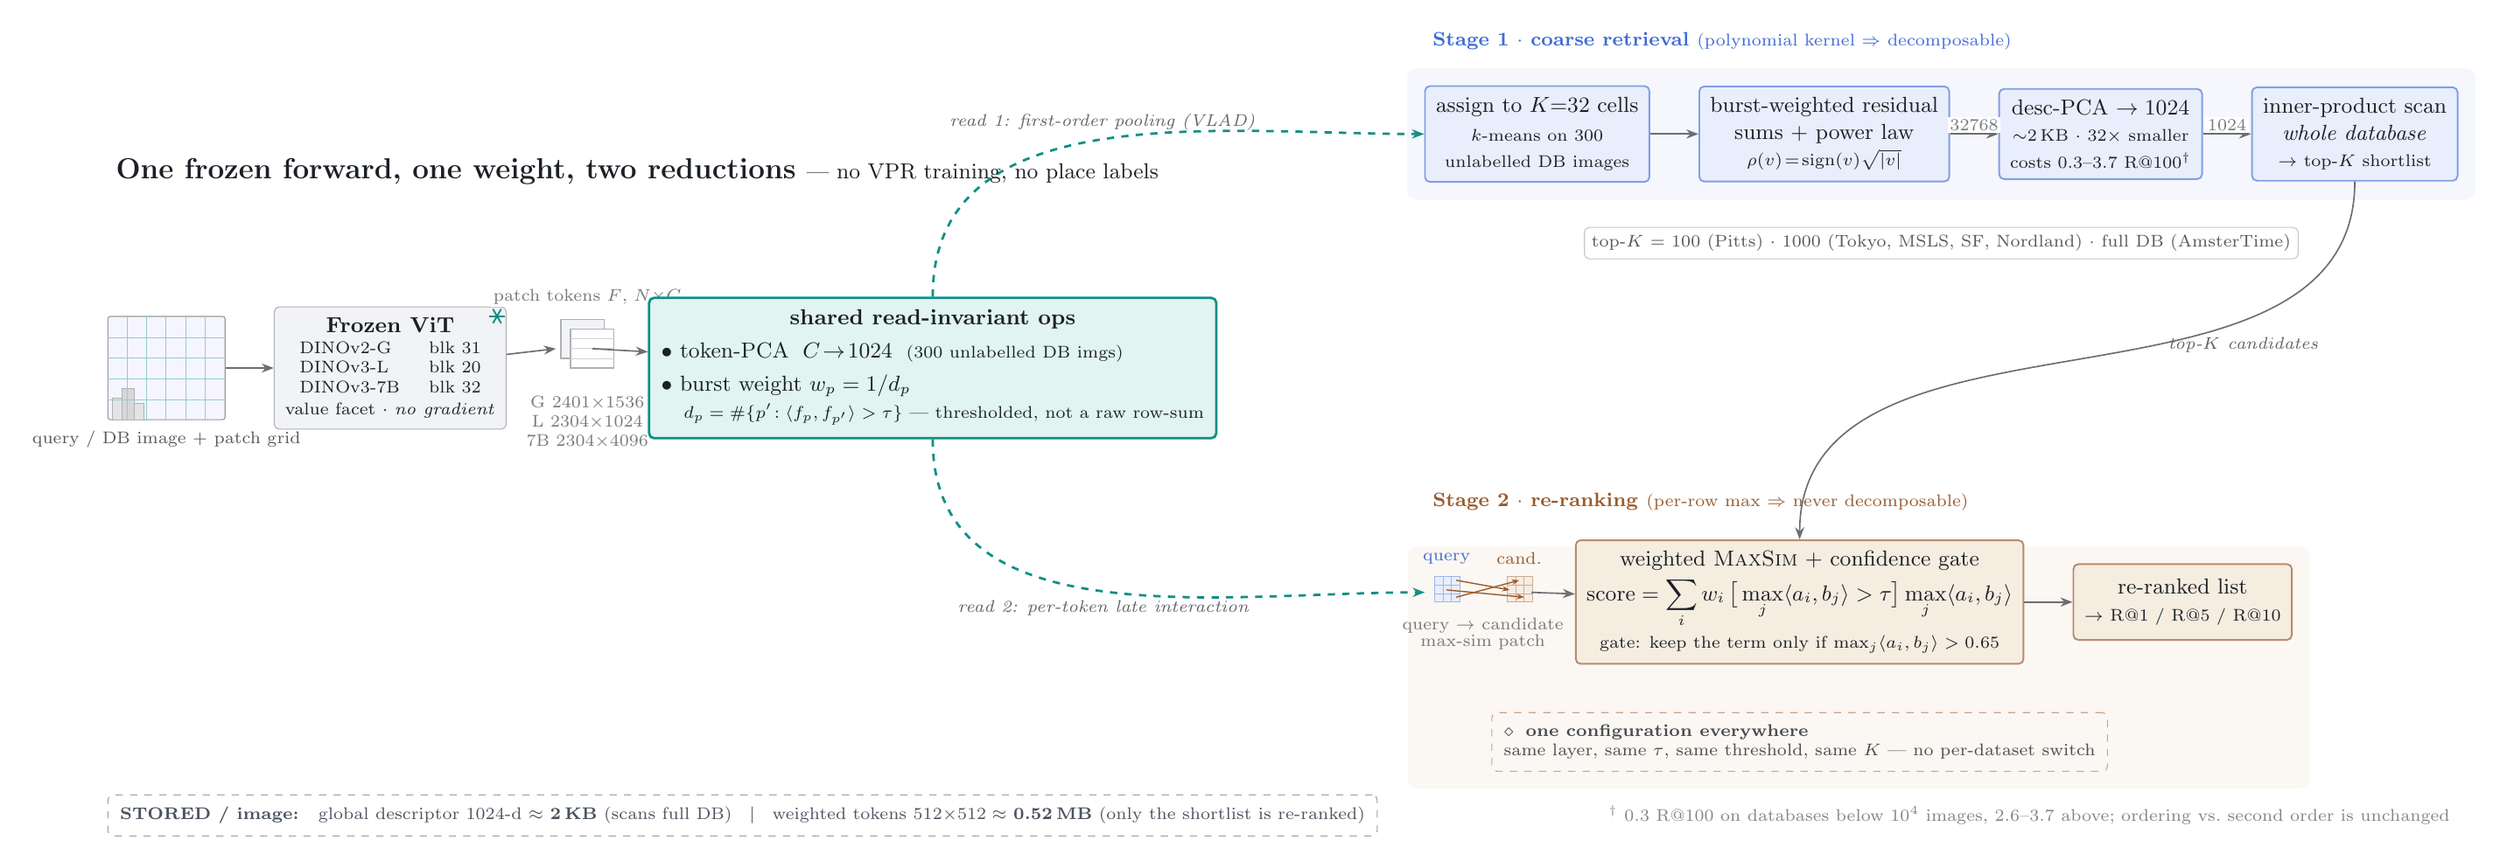
\begin{tikzpicture}[
  font=\small, text=ink, >=Stealth,
  box/.style={draw=ink!35, fill=greyb, rounded corners=2pt, align=center,
    inner sep=4.5pt, minimum height=9mm, font=\small},
  shbox/.style={draw=accent, line width=1pt, fill=accbg, rounded corners=2pt,
    align=center, inner sep=5pt, font=\small},
  s1box/.style={draw=sone!65, line width=0.7pt, fill=sonebg, rounded corners=2pt,
    align=center, inner sep=4.5pt, minimum height=11mm, font=\small},
  s2box/.style={draw=stwo!70, line width=0.7pt, fill=stwobg, rounded corners=2pt,
    align=center, inner sep=4.5pt, minimum height=11mm, font=\small},
  ar/.style={-{Stealth[length=5pt]}, draw=ink!65, line width=0.6pt},
  accar/.style={-{Stealth[length=5pt]}, draw=accent, line width=1pt, dashed},
  dimlbl/.style={font=\scriptsize, text=ink!60, fill=white, inner sep=1pt},
  lbl/.style={font=\scriptsize\itshape, text=ink!70},
  note/.style={font=\scriptsize, text=ink!75, align=center},
]

% ================= INPUT IMAGE + PATCH GRID =================
\node[draw=ink!45, fill=blue!4, minimum width=17mm, minimum height=15mm,
      inner sep=0, rounded corners=1pt] (imgN) at (0,0) {};
\draw[fill=ink!12, draw=ink!35, line width=0.4pt] ($(imgN.south west)+(2pt,0)$) rectangle ($(imgN.south west)+(6pt,9pt)$);
\draw[fill=ink!18, draw=ink!35, line width=0.4pt] ($(imgN.south west)+(6pt,0)$) rectangle ($(imgN.south west)+(11pt,13pt)$);
\draw[fill=ink!12, draw=ink!35, line width=0.4pt] ($(imgN.south west)+(11pt,0)$) rectangle ($(imgN.south west)+(15pt,7pt)$);
\foreach \i in {1,...,5}{\draw[accent!45,line width=0.3pt] ($(imgN.south west)+(\i*17/6*1mm,0)$)--($(imgN.north west)+(\i*17/6*1mm,0)$);}
\foreach \j in {1,...,4}{\draw[accent!45,line width=0.3pt] ($(imgN.south west)+(0,\j*3mm)$)--($(imgN.south east)+(0,\j*3mm)$);}
\node[note, below=1pt of imgN] {query / DB image + patch grid};

% ================= FROZEN BACKBONE =================
\node[box, right=7mm of imgN, minimum height=17mm, minimum width=31mm] (bb)
  {\textbf{Frozen ViT}\\[2pt]
   {\scriptsize\begin{tabular}{@{}ll@{}} DINOv2-G & blk 31\\ DINOv3-L & blk 20\\ DINOv3-7B & blk 32\end{tabular}}\\[1pt]
   {\scriptsize value facet $\cdot$ \emph{no gradient}}};
\coordinate (sf) at ($(bb.north east)+(-4pt,-4pt)$);
\foreach \a in {0,60,120}{\draw[accent,line width=0.7pt] ($(sf)+(\a:3.4pt)$)--($(sf)+(\a+180:3.4pt)$);}

% ================= TOKEN SLAB =================
\node[right=9mm of bb, inner sep=0] (tokanchor) {};
\fill[greyb, draw=ink!35, line width=0.5pt] ($(tokanchor.center)+(-4pt,4pt)$) rectangle ($(tokanchor.center)+(14pt,20pt)$);
\fill[white, draw=ink!35, line width=0.5pt] ($(tokanchor.center)+(0,0)$) rectangle ($(tokanchor.center)+(18pt,16pt)$);
\foreach \k in {1,2,3}{\draw[ink!20,line width=0.3pt] ($(tokanchor.center)+(0,\k*4pt)$) -- ($(tokanchor.center)+(18pt,\k*4pt)$);}
\node[dimlbl, anchor=south] at ($(tokanchor.center)+(7pt,25pt)$) {patch tokens $F$, $N{\times}C$};
\node[note, text=ink!60, anchor=north] (tokdims) at ($(tokanchor.center)+(7pt,-8pt)$)
  {\scriptsize G $2401{\times}1536$\\ L $2304{\times}1024$\\ 7B $2304{\times}4096$};

\draw[ar] (imgN) -- (bb);
\draw[ar] (bb) -- ($(tokanchor.center)+(-6pt,8pt)$);

% ================= SHARED OPS =================
\node[shbox, right=11mm of tokanchor, minimum width=35mm] (sh)
  {\textbf{shared read-invariant ops}\\[3pt]
   \begin{tabular}{@{}l@{}}
   $\bullet$ token-PCA $\;C\!\to\!1024$ \;{\scriptsize(300 unlabelled DB imgs)}\\[3pt]
   $\bullet$ burst weight $w_p=1/d_p$\\
   \quad{\scriptsize $d_p=\#\{p'\!:\langle f_p,f_{p'}\rangle>\tau\}$ --- thresholded, not a raw row-sum}
   \end{tabular}};
\draw[ar] ($(tokanchor.center)+(9pt,8pt)$) -- (sh);

% ================= STAGE 1 (TOP) =================
\node[s1box, minimum width=28mm, anchor=west] (c1) at ($(sh.east)+(3.0,3.4)$)
  {assign to $K{=}32$ cells\\[1pt] {\scriptsize $k$-means on 300}\\ {\scriptsize unlabelled DB images}};
\node[s1box, right=7mm of c1, minimum width=25mm] (c2)
  {burst-weighted residual\\ sums $+$ power law\\ {\scriptsize $\rho(v)\!=\!\mathrm{sign}(v)\sqrt{|v|}$}};
\node[s1box, right=7mm of c2, minimum width=28mm] (c3)
  {desc-PCA $\to 1024$\\ {\scriptsize $\sim$2\,KB $\cdot$ $32\times$ smaller}\\ {\scriptsize costs $0.3$--$3.7$ R@100$^\dagger$}};
\node[s1box, right=7mm of c3, minimum width=27mm] (c4)
  {inner-product scan\\ \emph{whole database}\\ {\scriptsize $\to$ top-$K$ shortlist}};
\draw[ar] (c1) -- (c2);
\draw[ar] (c2) -- node[dimlbl,above]{$32768$} (c3);
\draw[ar] (c3) -- node[dimlbl,above]{$1024$} (c4);

\coordinate (bandmid) at ($(c1.west)!0.5!(c4.east)$);
\node[anchor=west, font=\footnotesize\bfseries, text=sone] at (c1.west |- 0,4.75)
  {Stage 1 $\cdot$ coarse retrieval \textnormal{\scriptsize(polynomial kernel $\Rightarrow$ decomposable)}};
\node[anchor=north, note, draw=ink!25, fill=white, rounded corners=2pt, inner sep=3pt]
  at (bandmid |- 0,2.05)
  {\scriptsize top-$K$ = 100 (Pitts) $\cdot$ 1000 (Tokyo, MSLS, SF, Nordland) $\cdot$ full DB (AmsterTime)};

% ================= STAGE 2 (BOTTOM) =================
% MaxSim mini visual (zero-size anchor at its left)
\coordinate (mm) at ($(sh.east)+(3.15,-3.4)$);
\foreach \i in {0,1,2}\foreach \j in {0,1,2}{\fill[sonebg,draw=sone!50,line width=0.3pt] ($(mm)+(\i*3.5pt,\j*3.5pt)$) rectangle ($(mm)+(\i*3.5pt+3.5pt,\j*3.5pt+3.5pt)$);}
\foreach \i in {0,1,2}\foreach \j in {0,1,2}{\fill[stwobg,draw=stwo!50,line width=0.3pt] ($(mm)+(30pt+\i*3.5pt,\j*3.5pt)$) rectangle ($(mm)+(30pt+\i*3.5pt+3.5pt,\j*3.5pt+3.5pt)$);}
\draw[stwo,line width=0.5pt,-{Stealth[length=3pt]}] ($(mm)+(9pt,9pt)$) -- ($(mm)+(31pt,5pt)$);
\draw[stwo,line width=0.5pt,-{Stealth[length=3pt]}] ($(mm)+(9pt,2pt)$) -- ($(mm)+(35pt,9pt)$);
\draw[stwo,line width=0.5pt,-{Stealth[length=3pt]}] ($(mm)+(5pt,5pt)$) -- ($(mm)+(37pt,2pt)$);
\node[note, text=ink!60, anchor=north] at ($(mm)+(20pt,-3pt)$) {\scriptsize query $\to$ candidate\\[-1pt]\scriptsize max-sim patch};
\node[note, text=sone, anchor=south, font=\scriptsize] at ($(mm)+(5pt,12pt)$) {query};
\node[note, text=stwo, anchor=south, font=\scriptsize] at ($(mm)+(35pt,12pt)$) {cand.};

\node[s2box, minimum width=44mm, anchor=west] (r2) at ($(mm)+(58pt,0)$)
  {weighted \textsc{MaxSim} $+$ confidence gate\\[2pt]
   $\displaystyle \mathrm{score}=\sum_i w_i\,\big[\max_j\langle a_i,b_j\rangle>\tau\big]\max_j\langle a_i,b_j\rangle$\\[2pt]
   {\scriptsize gate: keep the term only if $\max_j\langle a_i,b_j\rangle>0.65$}};
\node[s2box, right=7mm of r2, minimum width=24mm] (r3)
  {re-ranked list\\ {\scriptsize $\to$ R@1 / R@5 / R@10}};
\draw[ar] ($(mm)+(40pt,4pt)$) -- (r2);
\draw[ar] (r2) -- (r3);

\node[anchor=west, font=\footnotesize\bfseries, text=stwo] at (c1.west |- 0,-1.95)
  {Stage 2 $\cdot$ re-ranking \textnormal{\scriptsize(per-row max $\Rightarrow$ never decomposable)}};

% 说明:原本这里有一个 "optional (AmsterTime only) ZCA whitening" 方框,已删除 ——
% 那是逐数据集开关,与 \S\ref{sec:transfer} 主张的"没有逐集开关"直接冲突。
\node[draw=stwo!55, dashed, rounded corners=2pt, fill=stwobg!40, inner sep=5pt,
      font=\scriptsize, align=left, text=ink!80, anchor=north] (zca) at (r2.south |- 0,-5.0)
  {$\diamond$\; \textbf{one configuration everywhere}\\
   same layer, same $\tau$, same threshold, same $K$ --- no per-dataset switch};

% ================= SHARED (two reads) ARROWS =================
\draw[accar] (sh.north) to[out=90,in=180] node[lbl,above,pos=0.5]{read 1: first-order pooling (VLAD)} (c1.west);
\draw[accar] (sh.south) to[out=-90,in=180] node[lbl,below,pos=0.5]{read 2: per-token late interaction} ($(mm)+(-4pt,4pt)$);
\draw[ar] (c4.south) to[out=-90,in=90] node[lbl,right,pos=0.4]{top-$K$ candidates} (r2.north);

% ================= STORAGE + FOOTNOTE =================
\node[anchor=west, draw=store!55, dashed, rounded corners=2pt, inner sep=5pt,
      font=\scriptsize, align=left, text=store] (stor) at (imgN.west |- 0,-6.5)
  {\textbf{STORED / image:}\;\; global descriptor $1024$-d $\approx$ \textbf{2\,KB} (scans full DB) \;\;$|$\;\;
   weighted tokens $512{\times}512\approx$ \textbf{0.52\,MB} (only the shortlist is re-ranked)};
\node[anchor=east, note, text=ink!55] at (c4.east |- 0,-6.5)
  {\scriptsize $^\dagger$ $0.3$ R@100 on databases below $10^4$ images, $2.6$--$3.7$ above; ordering vs.\ second order is unchanged};

% ================= TITLE =================
\node[anchor=south west, font=\large\bfseries, text=ink] at (imgN.west |- 0,2.55)
  {One frozen forward, one weight, two reductions
   \textnormal{\normalfont\small--- no VPR training, no place labels}};

% ================= BANDS =================
\begin{scope}[on background layer]
  \node[fill=sonebg!45, rounded corners=4pt, fit=(c1)(c4), inner sep=7pt] {};
  \coordinate (mmA) at ($(mm)+(-4pt,14pt)$);
  \coordinate (mmB) at ($(mm)+(40pt,-16pt)$);
  \node[fill=stwobg!45, rounded corners=4pt, fit=(mmA)(mmB)(r3)(zca), inner sep=7pt] {};
\end{scope}

\end{tikzpicture}
}  % TikZ version, swapped out for a trial
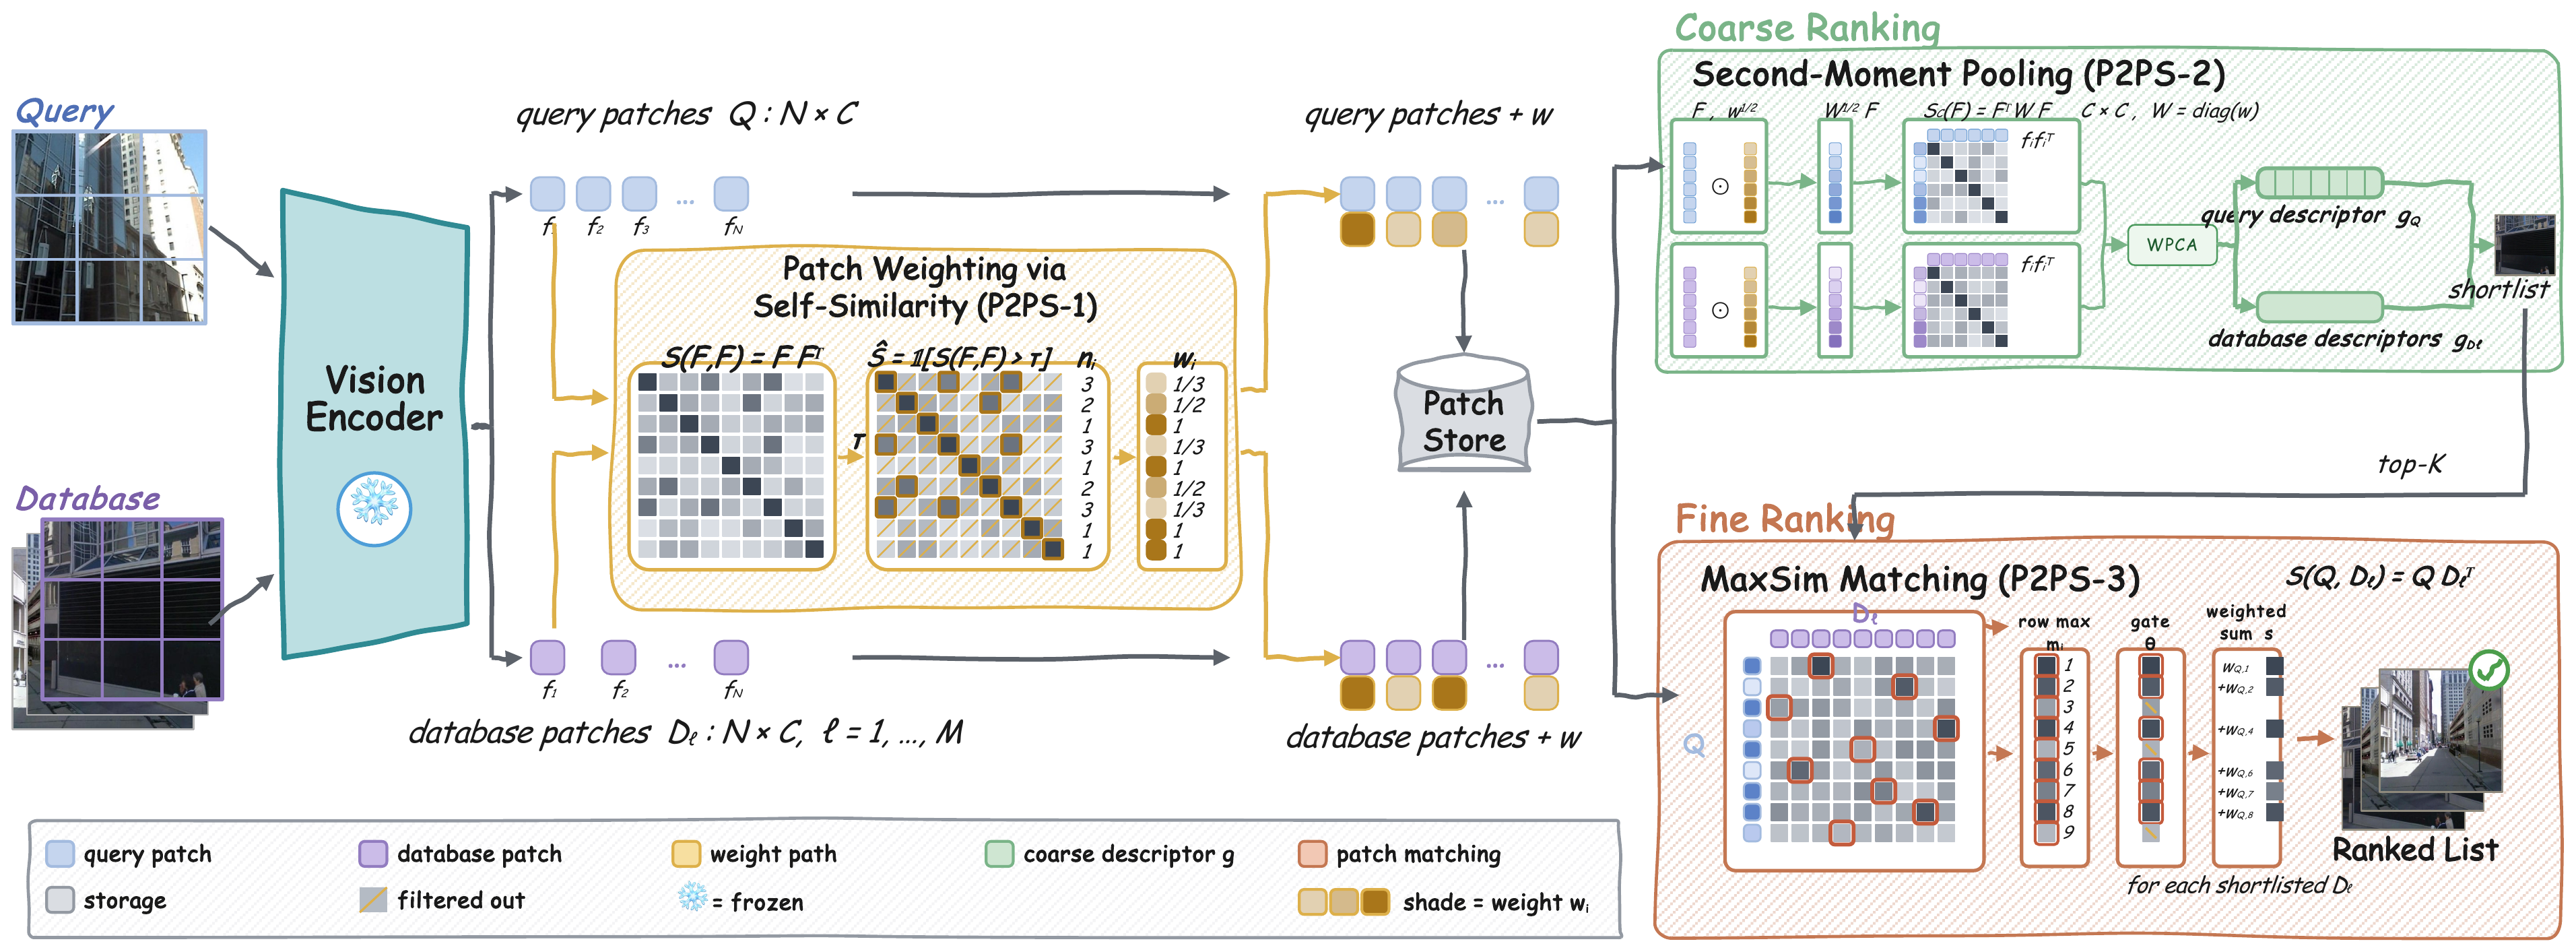
\includegraphics[width=\textwidth]{figures/method_fig_ppt.png}
\caption{\textbf{One frozen forward, one weight, two reductions.} Thresholding and row-summing $G_N{=}FF^{\top}$ gives $w_i{=}1/n_i$, which weights both stages and prunes the store. Stage 1 scans the whitened second moment $G_C{=}F^{\top}WF$; stage 2 re-ranks its shortlist by the row-max reduction of $S{=}QD^{\top}$.}
\label{fig:method}
\end{figure}

\subsection{Tokens}
\label{sec:prelim}
An image is passed through a frozen DINOv2/DINOv3 backbone, and we take the value facet of a fixed block, the output of its value projection, which \citet{vitfacets} introduced as a dense descriptor and \citet{effovpr} adopted for VPR. A PCA is fitted across patch tokens collected from a few hundred unlabelled database images and is then applied to every token, reducing it to $C{=}512$ channels; each token is $\ell_2$-normalized before and after. This gives $N$ unit-norm patch features per image, written $\mathbf f_1,\dots,\mathbf f_N$ and stacked row-wise as $F$. Two kinds of similarity follow: within one image, $G_{ij}=\mathbf f_i^{\top}\mathbf f_j$, and between a query and a candidate, $S_{ij}=\mathbf q_i^{\top}\mathbf d_j$. Block, facet and shortlist depth are swept in Appendix~\ref{app:hyper}.

\subsection{The weight}
\label{sec:feat}
A patch of sky, or one window in a facade of identical windows, appears many times in the same image, and every copy is counted again. We want ten nearly identical sky patches to contribute about as much as one unique patch, rather than ten times as much. We therefore give each patch a weight before either stage uses it.

For token $i$, we want the total weight of the tokens similar to it to be approximately constant. If $G_{ij}$ measures token similarity, this condition reads
\begin{equation}\label{eq:demo}
  \sum_j G_{ij}\,w_j = 1,
  \qquad\text{or in matrix form}\qquad
  G\mathbf w=\mathbf 1,
\end{equation}
which is the democratic-weighting condition of \citet{democratic} and \citet{gmp}. We impose it not on $G$ but on its thresholded version $\hat G_{ij}=\mathbb 1[\,G_{ij}>\tau\,]$, which counts near-duplicates instead of grading them. The condition then has a closed-form solution,
\begin{equation}\label{eq:weight}
  w_i=\frac{1}{n_i},
  \qquad
  n_i=\sum_j \hat G_{ij},
\end{equation}
the reciprocal of the number of patches in the image that resemble patch $i$: a sky patch that appears twenty times receives one twentieth of the weight of a patch that appears once. Appendix~\ref{app:ridge} derives this and relates it to the regularized solution of \citet{gmp}. The only constant is the threshold $\tau$, fixed at $0.5$ for every backbone and dataset. Figure~\ref{fig:vis-c1} draws the near-duplicate groups at that threshold.

\subsection{First stage}
\label{sec:global}
Stage 1 needs a fixed-size descriptor for each image so that all database images can be searched efficiently. We obtain it by weighted second-order pooling of the patch features.

Take one patch $\mathbf q$ from the query and one patch $\mathbf d$ from a candidate. Their similarity is $\mathbf q^{\top}\mathbf d$, and its square can be rewritten as $(\mathbf q^{\top}\mathbf d)^2=\langle\,\mathbf q\mathbf q^{\top},\ \mathbf d\mathbf d^{\top}\,\rangle$, a comparison of two matrices, each built from one image alone. Summing over all patch pairs with the weights of \S\ref{sec:feat} therefore separates into a single comparison between two per-image matrices,
\begin{equation}\label{eq:so-deriv}
  \sum_{i,j} w_{Q,i}\,w_{D,j}\,\big(\mathbf q_i^{\top}\mathbf d_j\big)^{2}
  =\big\langle\, G_C(Q),\ G_C(D)\,\big\rangle,
  \qquad
  G_C(F)=\frac{1}{\sum_i w_i}\sum_i w_i\,\mathbf f_i\mathbf f_i^{\top}.
\end{equation}
$G_C$ records how the image's features co-occur across channels, with no reference to where in the image they appeared, which is what lets two views of a place match under a change of viewpoint, and it retains far more than an average of the features would (Appendix~\ref{app:coarsegrid}). Other powers of the similarity factorize in the same way, as Appendix~\ref{app:factorize} works out.

The stored descriptor is $G_C$ flattened, with a square root applied to each entry, and the result $\ell_2$-normalized:
\begin{equation}\label{eq:stage1}
  \psi(F)\;=\;\frac{\rho\big(\operatorname{vec}(G_C(F))\big)}{\lVert\rho\big(\operatorname{vec}(G_C(F))\big)\rVert_2},
  \qquad
  \rho(u)=\operatorname{sign}(u)\sqrt{|u|}.
\end{equation}
The square root is the power normalization of \citet{improvedfisher}, standard for Fisher vectors and VLAD \citep{allvlad}. Its purpose is the same as the weight's. A repeated element makes a few entries of the descriptor very large, and those entries then dominate the comparison between two images. Taking square roots pulls the large entries down and lets the rest of the descriptor count. The weight acts on patches before pooling and the square root acts on the descriptor after it, so the two do not overlap.

The descriptor is reduced to $2048$ dimensions by a whitened PCA, again fitted on the deployment database, and the scan returns the $P{=}\min(1000,|\mathcal{D}|)$ best candidates. The same weight also decides what to store: each image keeps its $1024$ highest-weight patches, with the weights computed on the full set and carried along (\S\ref{sec:stage1abl}). Nothing is fitted outside $\mathcal{D}$; Figure~\ref{fig:patchcov} shows the stored matrix.

\subsection{Second stage}
\label{sec:core}
For each query patch we find its most similar patch in the candidate image and sum those similarities,
\begin{equation}\label{eq:stage2}
  s(Q,D)=\sum_{i=1}^{N_Q} w_{Q,i}\;\mathbb 1[\,m_i>\theta\,]\;m_i
  \qquad\text{with}\qquad
  m_i=\max_{j} S_{ij},
\end{equation}
which is the \textsc{MaxSim} late-interaction rule of \citet{colbert}, weighted as in \S\ref{sec:feat}. Sky, pedestrians and occluders have no counterpart in the other image, and \textsc{MaxSim} would still score them at their best accidental match, so a patch counts only if its best match clears a confidence threshold $\theta$, fixed at $0.65$ throughout; Appendix~\ref{app:calib} gives the sweep and the reasoning behind it.

Unlike the first stage, \textsc{MaxSim} cannot be represented by a single fixed-size image descriptor, so we apply it only to the shortlisted candidates, which keeps it affordable; Appendix~\ref{app:nofactor} explains why no such descriptor exists. A method that stores one descriptor per image is therefore denied this stage, and must train its pooling until that single vector separates places on its own \citep{netvlad}. The tables denote our rule \textsc{selfw\_conf}, and Figure~\ref{fig:vis-m1} draws its surviving matches. A variant \textsc{mnn\_selfw65} additionally requires each match to be mutual and counts weighted inliers instead of summing similarities; Appendix~\ref{app:effo-matched} runs both against \textsc{EffoVPR}'s attention-selected rule on an identical shortlist and identical features.


\section{Evaluation}
\label{sec:exp}
\begin{figure}[t]
\centering
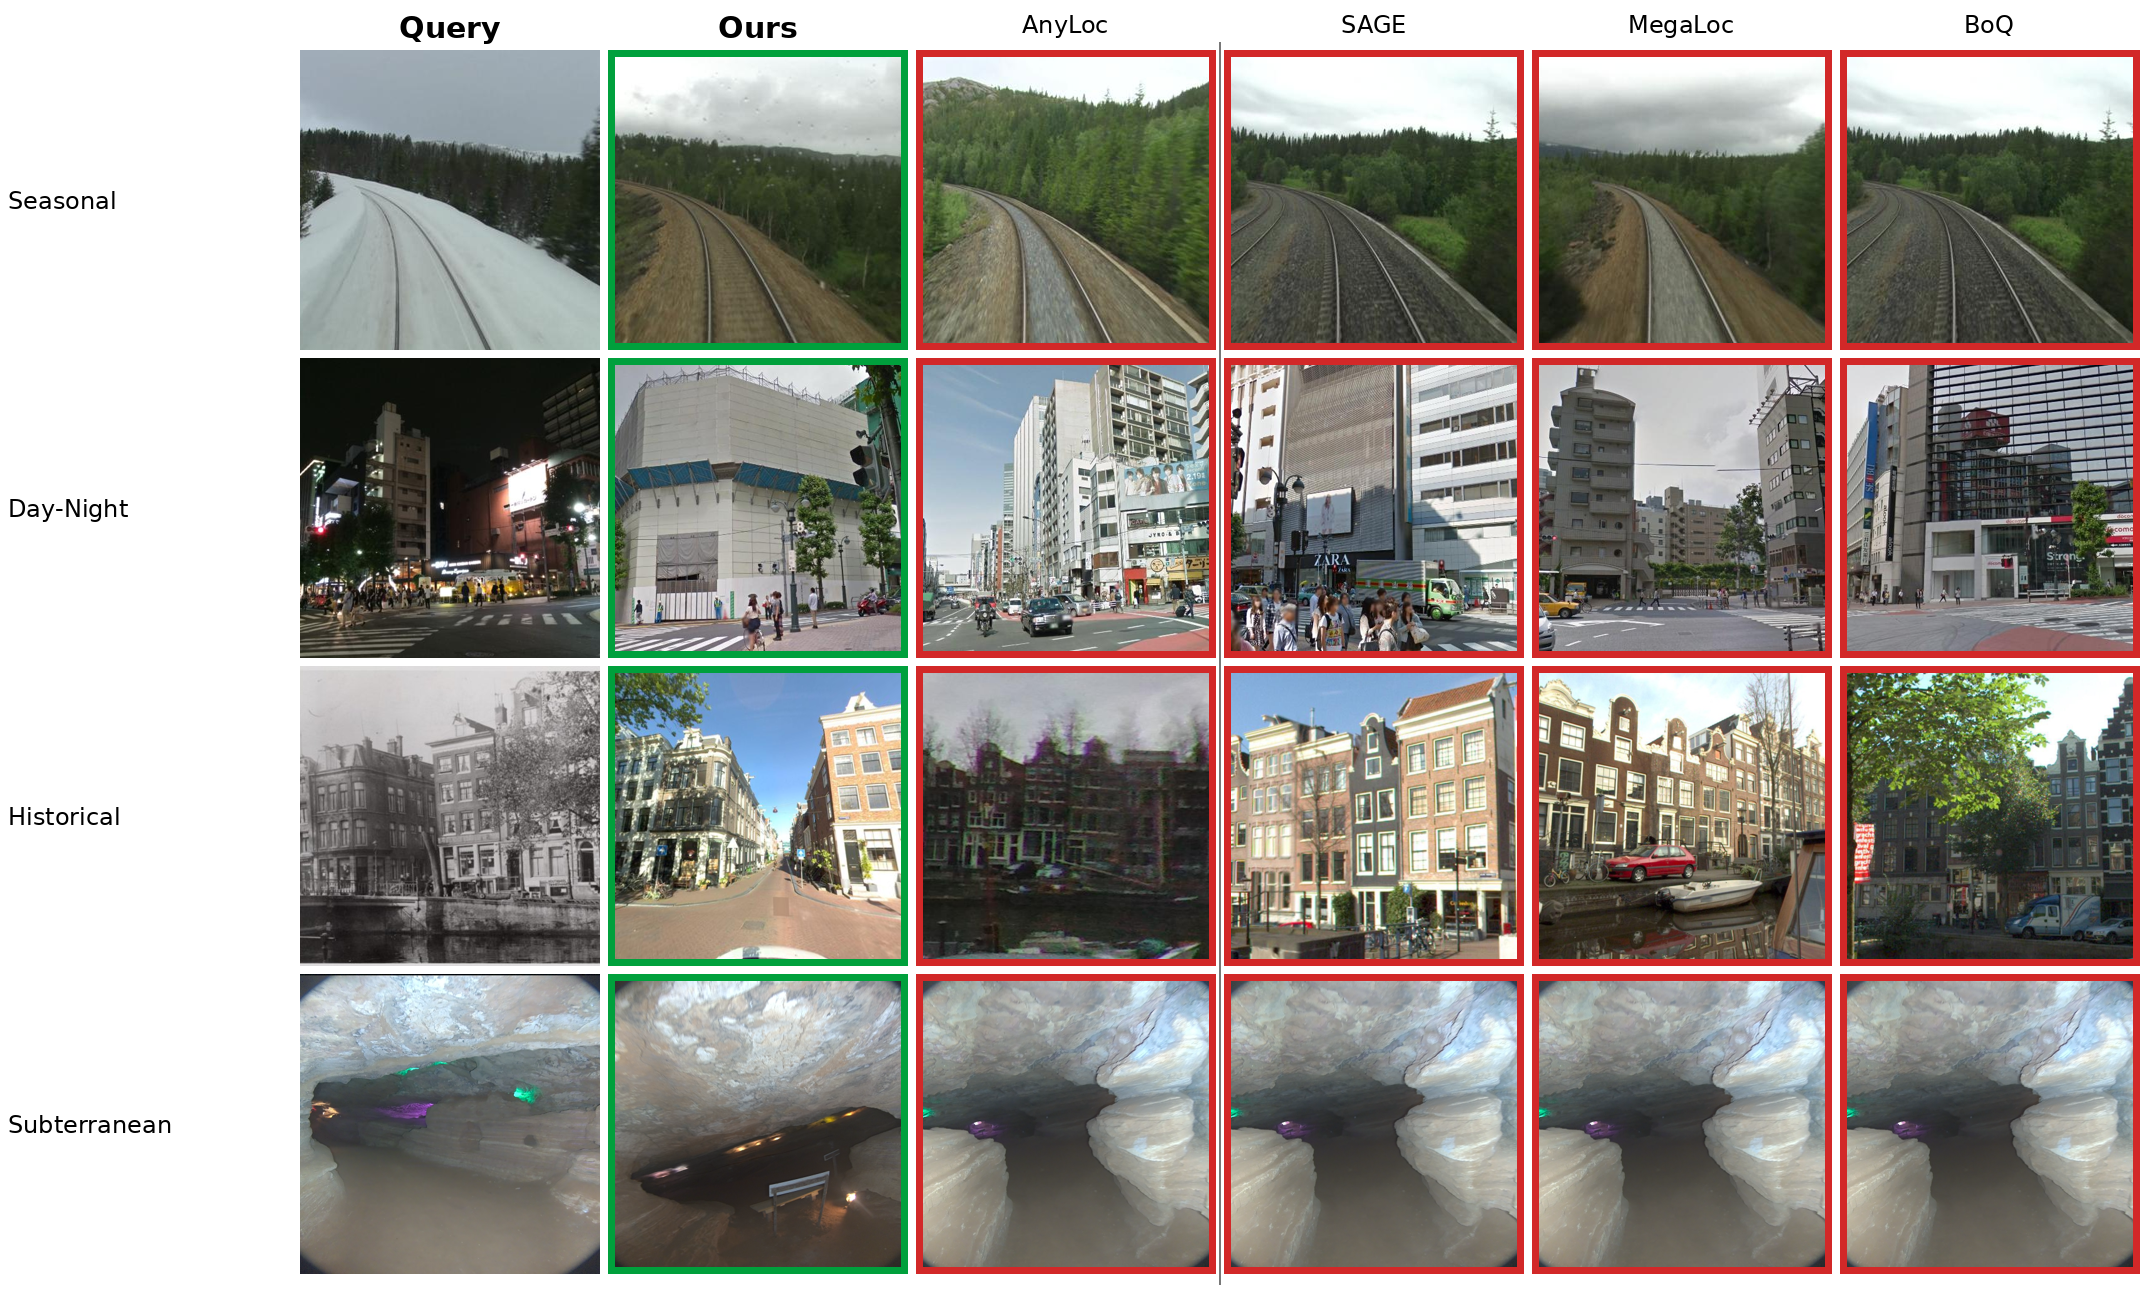
\includegraphics[width=0.82\textwidth]{figures/fig_qualitative.png}
\caption{\textbf{Rank-1 retrievals across benchmark families.} Each method at its own single stage; a green border marks a correct rank-1, red an incorrect one. Training-free methods above the line, the three strongest trained baselines below. Queries are drawn automatically from those our pipeline retrieves correctly, on five axes the one whose correct image sits furthest down every trained baseline's ranking, on the viewpoint axis one the strongest trained baseline still gets right, and on the degraded axis one AnyLoc gets right.}
\label{fig:qual}
\end{figure}

\subsection{Setup and protocol}
\label{sec:setup}

\begin{table}[t]
\caption{\textbf{The thirteen benchmarks.} What each one asks of a place representation. Splits, database and query counts and ground-truth distances are in Appendix~\ref{app:protocol}.}
\label{tab:datasets}
\centering
{\footnotesize\setlength{\tabcolsep}{4pt}%
\begin{tabular}{ll}
\toprule
Benchmark & What it tests \\
\midrule
\multicolumn{2}{l}{\emph{Urban, street level}} \\
Pitts30k, Pitts250k & viewpoint change in a dense city survey \\
Tokyo 24/7 & the same places by day, at dusk and at night \\
MSLS-val & a moving camera across cities, seasons and weather \\
St Lucia & a vehicle repeating a suburban route \\
Oxford RobotCar & a vehicle repeating a route months apart \\
Nordland & one railway line in four seasons, no viewpoint change \\
AmsterTime & historical photographs against present-day ones \\
\midrule
\multicolumn{2}{l}{\emph{Beyond street level}} \\
Hawkins, Laurel Caverns & subterranean corridors, little texture, poor light \\
17 Places, Baidu Mall & indoor scenes that repeat themselves \\
Gardens Point & an indoor route walked by day and by night \\
VP-Air, Nardo-Air, Nardo-Air R & aerial imagery, the last one rotated \\
Mid-Atlantic Ridge & deep-sea imagery from a hydrothermal vent \\
\bottomrule
\end{tabular}%
}
\end{table}

\subsection{Comparison with state-of-the-art}
\label{sec:sota}

\begin{table}[t]
\caption{\textbf{All methods on all seventeen benchmarks.} Recall@1, one deployed configuration throughout; the urban block re-ranks $1024$ tokens per image, the environment block all $2{,}304$. \emph{Dim} is the first-stage descriptor dimensionality, as evaluated. \textsc{CLS token} is the frozen DINOv2-L class token retrieved by cosine. Baseline cells are published numbers, or our run of the released code where the paper omits the benchmark; ``---'' marks a run not yet complete. $^{d}$AnyLoc's VP-Air figure may omit the $10{,}000$ distractors ours carries. $^{\dagger}$after the method's own re-ranker; $^{\ddag}$without the cross-image encoder. Bold $=$ best, \underline{underline} $=$ second, within each block.}
\label{tab:breadth}
\centering
{\scriptsize\setlength{\tabcolsep}{2.0pt}\renewcommand{\arraystretch}{0.9}%
\begin{tabular}{ll ccccccccc|c}
\toprule
\multicolumn{12}{l}{\emph{Standard benchmarks (urban)}} \\
Method & Dim & Pitts250k & Pitts30k & Tokyo24/7 & MSLS-val & Nordland & St Lucia & Oxford & AmsterTime & & mean \\
\midrule
\multicolumn{12}{l}{\emph{Trained or fine-tuned}} \\
NetVLAD & 32768 & 81.5 & 82.1 & 54.9 & 53.1 & 6.4 & 49.9 & 34.6 & 20.6 &  & 47.9 \\
SFRS & 4096 & 90.7 & 70.9 & 85.4 & 59.3 & 8.8 & 58.6 & 29.3 & 19.3 &  & 52.8 \\
CosPlace & 2048 & 92.2 & 90.9 & 87.3 & 87.7 & 63.0 & 99.9 & 79.1 & 49.7 &  & 81.2 \\
MixVPR & 4096 & 94.6 & 91.6 & 86.3 & 88.0 & 76.6 & 99.6 & 90.6 & 40.9 &  & 83.5 \\
EigenPlaces & 2048 & 94.1 & 92.5 & 93.0 & 89.1 & 63.6 & 99.5 & 89.5 & 48.9 &  & 83.8 \\
R2Former$^{\dagger}$ & 256 & 93.2 & 91.1 & 88.6 & 89.7 & 60.5 & 99.7 & 92.7 & 29.5 &  & 80.6 \\
SALAD & 8448 & 95.1 & 92.4 & 94.6 & 92.2 & 86.5 & \textbf{100.0} & 97.9 & 58.4 &  & 89.6 \\
CricaVPR$^\ddag$ & 10752 & 94.6 & 91.8 & 90.2 & 89.2 & 80.5 & 99.8 & 98.4 & 49.0 &  & 86.7 \\
SelaVPR$^{\dagger}$ & 1024 & 95.7 & 92.8 & 94.0 & 90.8 & 85.2 & 99.8 & 99.0 & 50.3 &  & 88.4 \\
BoQ & 12288 & 96.6 & 93.7 & 98.1 & 93.8 & 90.6 & \textbf{100.0} & 99.5 & 63.0 &  & 91.9 \\
CliqueMining & 8448 & 95.2 & 92.6 & 96.8 & 94.2 & 95.9 & \textbf{100.0} & 98.4 & 57.7 &  & 91.4 \\
SuperVLAD$^\ddag$ & 3072 & 95.2 & 92.6 & 93.7 & 91.5 & 79.2 & 99.9 & \textbf{100.0} & 54.7 &  & 88.3 \\
VLAD-BuFF & 4096 & 95.6 & 92.5 & 96.5 & 92.4 & 84.9 & \textbf{100.0} & 99.0 & 61.4 &  & 90.3 \\
SelaVPR++$^{\dagger}$ & 2048 & 96.7 & 94.4 & 98.1 & \textbf{94.5} & \textbf{97.2} & \textbf{100.0} & 99.5 & 61.2 &  & 92.7 \\
MegaLoc & 8448 & 96.4 & 94.1 & 96.5 & 91.0 & 94.3 & \textbf{100.0} & 99.0 & 62.5 &  & 91.7 \\
FoL$^{\dagger}$ & 8448 & \textbf{97.0} & \underline{94.5} & \underline{98.4} & 93.5 & 92.6 & 99.9 & \textbf{100.0} & \underline{70.1} &  & \underline{93.2} \\
SAGE$^\ddag$ & 8448 & \underline{96.8} & \textbf{94.7} & 97.8 & \underline{94.5} & 95.1 & \underline{99.9} & 99.5 & 66.0 &  & 93.0 \\
\midrule
\multicolumn{12}{l}{\emph{Training-free}} \\
CLS token & 1024 & 80.3 & 78.7 & 46.0 & 37.8 & 15.9 & 81.5 & 25.6 & 45.8 &  & 51.5 \\
GeM & 1024 & 80.4 & 78.5 & 69.8 & 36.0 & 15.0 & 74.2 & 71.7 & 27.9 &  & 56.7 \\
AnyLoc & 49152 & 81.5 & 87.7 & 90.5 & 49.2 & 20.2 & 96.2 & \underline{99.5} & 44.6 &  & 71.2 \\
EffoVPR-ZS$^{\dagger}$ & 1024 & 93.4 & 89.4 & 90.8 & 70.3 & 57.9 & 97.8 & 77.0 & 65.8 &  & 80.3 \\
SegVLAD-PreT & 49152 & --- & 86.7 & --- & --- & --- & --- & 73.8 & 62.4 &  & --- \\
\midrule
Ours\,\emph{v2}$^{\dagger}$ & 2048 & 95.7 & 92.5 & 97.5 & 89.0 & 83.0 & 99.1 & 99.0 & 68.1 &  & 90.5 \\
Ours\,\emph{v3}$^{\dagger}$ & 2048 & 96.1 & 93.7 & \textbf{98.4} & 89.3 & \underline{96.6} & 99.7 & 99.0 & \textbf{73.6} &  & \textbf{93.3} \\
\midrule\midrule
\multicolumn{12}{l}{\emph{Nine environments}} \\
Method & Dim & Hawk & Laurel & 17Pl & Gard & Baidu & N-Air & N-AirR & VP-Air & M-Atl & mean \\
\midrule
\multicolumn{12}{l}{\emph{Trained or fine-tuned}} \\
NetVLAD & 32768 & 38.1 & 42.9 & 63.8 & 66.0 & 57.8 & 9.9 & 39.4 & 14.7 & 26.7 & 39.9 \\
SFRS & 4096 & 29.7 & 21.4 & 59.1 & 55.0 & 51.3 & 0.0 & 47.9 & 9.4 & 9.9 & 31.5 \\
CosPlace & 2048 & 33.9 & 25.9 & 63.3 & 84.5 & 47.1 & 0.0 & 76.1 & 10.4 & 32.7 & 41.5 \\
MixVPR & 4096 & 26.3 & 32.1 & 63.8 & 92.0 & 68.4 & 39.4 & 78.9 & 12.9 & 24.8 & 48.7 \\
EigenPlaces & 2048 & 28.8 & 27.7 & 63.8 & 86.0 & 66.6 & 12.7 & \textbf{100.0} & 13.1 & 29.7 & 47.6 \\
R2Former$^{\dagger}$ & 256 & 17.8 & 30.4 & 63.8 & 84.0 & 74.7 & 26.8 & 83.1 & 15.0 & 22.8 & 46.5 \\
SALAD & 8448 & 38.1 & 46.4 & 64.3 & 96.5 & 69.9 & 53.5 & 94.4 & 24.0 & 15.8 & 55.9 \\
CricaVPR$^\ddag$ & 10752 & 28.0 & 34.8 & 64.0 & 94.0 & 65.8 & 45.1 & \textbf{100.0} & 19.9 & 27.7 & 53.3 \\
SelaVPR$^{\dagger}$ & 1024 & 25.4 & 53.6 & 63.3 & 94.5 & 68.5 & 59.1 & 83.1 & 32.6 & 21.8 & 55.8 \\
BoQ & 12288 & 33.9 & 60.7 & 64.3 & \underline{98.0} & 77.4 & 62.0 & 91.5 & 29.5 & 35.6 & 61.4 \\
CliqueMining & 8448 & 22.9 & 38.4 & \underline{65.3} & 93.0 & 69.1 & 62.0 & 84.5 & 22.9 & 35.6 & 54.9 \\
SuperVLAD$^\ddag$ & 3072 & 37.3 & 51.8 & 64.8 & 95.5 & 70.3 & 14.1 & 88.7 & 23.8 & 13.9 & 51.1 \\
VLAD-BuFF & 4096 & 37.3 & 33.9 & 64.5 & 96.5 & 76.4 & 57.7 & 88.7 & 33.3 & 27.7 & 57.4 \\
SelaVPR++$^{\dagger}$ & 2048 & 21.2 & 35.7 & 65.0 & 95.5 & 73.6 & 81.7 & 87.3 & 42.7 & 27.7 & 58.9 \\
MegaLoc & 8448 & 37.3 & 55.4 & 64.8 & 95.5 & 79.4 & \underline{85.9} & 81.7 & 45.6 & \textbf{40.6} & 65.1 \\
FoL$^{\dagger}$ & 8448 & 36.4 & 54.5 & \underline{65.3} & 97.0 & 78.9 & 77.5 & \underline{98.6} & 46.7 & 25.7 & 64.5 \\
SAGE$^\ddag$ & 8448 & 27.1 & 46.4 & 64.0 & 93.5 & 74.6 & \underline{85.9} & 84.5 & 39.1 & 24.8 & 60.0 \\
\midrule
\multicolumn{12}{l}{\emph{Training-free}} \\
CLS token & 1024 & 26.3 & 50.9 & 61.1 & 75.0 & 43.1 & 56.3 & 76.1 & 38.0 & 24.8 & 50.2 \\
GeM & 1024 & 56.8 & 50.9 & 64.0 & 89.5 & 46.2 & 81.7 & 85.9 & 42.2 & 23.8 & 60.1 \\
AnyLoc & 49152 & \underline{65.2} & 61.6 & 65.0 & 95.5 & 75.2 & 76.1 & 85.9 & 66.7$^{d}$ & 34.6 & 69.5 \\
EffoVPR-ZS$^{\dagger}$ & 1024 & 38.1 & 67.0 & \textbf{65.5} & 97.5 & 75.9 & 83.1 & 88.7 & 65.7 & 36.6 & 68.7 \\
SegVLAD-PreT & 49152 & 56.8 & 26.8 & 64.8 & 91.5 & 78.5 & 45.1 & 40.9 & 69.8 & 22.8 & 55.2 \\
\midrule
Ours\,\emph{v2} & 2048 & \textbf{67.0} & \textbf{83.0} & \textbf{65.5} & \textbf{99.5} & \textbf{84.5} & 83.1 & 94.4 & \underline{72.1} & \underline{37.6} & \underline{76.3} \\
Ours\,\emph{v3} & 2048 & 61.0 & \underline{75.9} & \underline{65.3} & \textbf{99.5} & \underline{83.5} & \textbf{91.5} & 97.2 & \textbf{77.6} & \underline{37.6} & \textbf{76.6} \\
\bottomrule
\end{tabular}%
}
\end{table}

\label{sec:ood}

\subsection{Ablation study}
\label{sec:swap}

\begin{table}[t]
\caption{\textbf{Which patch-importance signal.} Pitts30k, $6816$ queries, DINOv2-G layer $31$, weighted \textsc{MaxSim} over an AnyLoc top-$100$ pool. Every row changes only $w$. \emph{Source} names the work the signal is taken from.}
\label{tab:w-signal}
\centering
{\footnotesize
\begin{tabular}{ll c l}
\toprule
Signal for $w$   &   Source   &  R@1 &   \\
\midrule
none (bare \textsc{MaxSim})   &   ---   &  87.62 &   baseline \\
\midrule
\textbf{self-similarity, down-weighted}   &   this work   &  \textbf{93.03} &   best \\
class-token attention, up-weighted    &    \citep{effovpr}    &  92.62 &    close second \\
patch-graph centrality, up-weighted    &    SAP    &  90.44 &    works, weaker \\
\midrule
patch-graph centrality, \emph{down}-weighted   &   ---   &  83.94 &   direction reversed \\
token norm, up-weighted    &    \citep{registers}    &  87.72 &    neutral \\
token norm, down-weighted    &    \citep{registers}    &  87.53 &    neutral \\
inverse document frequency    &    Video Google    &  86.53 &    below baseline \\
cross-referencing    &    DeepEMD    &  81.78 &    below baseline \\
rapid spatial verification    &    \citep{patchnetvlad}    &  84.24 &    below baseline \\
\bottomrule
\end{tabular}%
}\end{table}

\begin{table}[t]
\caption{\textbf{Our second stage on other methods' first stages.} Each figure is what the method publishes, after its own re-ranker in the upper block and from its global descriptor in the lower; the subscript is the change under \eqref{eq:stage2}, replacing that re-ranker or added where there is none. Backbone, resolution and shortlist stay the method's own.}
\label{tab:stage2swap}
\centering
{\scriptsize\setlength{\tabcolsep}{2pt}%
\resizebox{\textwidth}{!}{%
\begin{tabular}{llccccccccc|c}
\toprule
& & Degr.\ & SubT & \multicolumn{3}{c}{Indoor} & \multicolumn{3}{c}{Aerial} & UW & \\
\cmidrule(lr){3-11}
Method   &   Backbone   &   Hawk   &   Laurel   &  17Pl &   Gard   &   Baidu   &   N-Air   &   N-AirR   &   VP-Air   & M-Atl &   mean \\
\midrule
\multicolumn{12}{l}{\emph{Replacing each method's own re-ranking stage}} \\
FoL            & DINOv2-L   & 36.4\dlt{+14.4} & 54.5\dlt{+18.7} & 65.3\dlt{-0.5} & 97.0\dlt{+1.0} & 78.9\dlt{+2.4} & 77.5\dlt{+4.2} & 98.6\dlt{-4.2} & 46.7\dlt{+10.1} & 25.7\dlt{+3.0} & 64.5\dltg{+5.5} \\
SelaVPR++      & DINOv2-L   & 21.2\dlt{+44.9} & 35.7\dlt{+39.3} & 65.0\dlt{-0.0} & 95.5\dlt{+3.0} & 73.6\dlt{+8.0} & 81.7\dlt{-5.6} & 87.3\dlt{+2.8} & 42.7\dlt{+25.0} & 27.7\dlt{-4.9} & 58.9\dltg{+12.5} \\
SelaVPR        & DINOv2-L   & 25.4\dlt{+38.2} & 53.6\dlt{+13.4} & 63.3\dlt{+2.5} & 94.5\dlt{+1.5} & 68.5\dlt{+7.5} & 59.1\dlt{+1.5} & 83.1\dlt{+1.4} & 32.6\dlt{+23.5} & 21.8\dlt{-2.0} & 55.8\dltg{+9.7} \\
R2Former       & DeiT-S     & 17.8\dlt{+22.9} & 30.4\dlt{+16.1} & 63.8\dlt{+0.7} & 84.0\dlt{-3.5} & 74.7\dlt{+0.6} & 26.8\dlt{+5.6} & 83.1\dlt{-1.4} & 15.0\dlt{+2.8} & 22.8\dlt{+6.9} & 46.5\dltg{+5.6} \\
\midrule
\multicolumn{12}{l}{\emph{Added to methods that provide no re-ranking stage}} \\
SALAD                & DINOv2-B   & 38.1\dlt{+24.6} & 46.4\dlt{+25.9} & 64.3\dlt{+1.0} & 96.5\dlt{+3.0} & 69.9\dlt{+12.1} & 53.5\dlt{+29.6} & 94.4\dlt{+1.4} & 24.0\dlt{+22.1} & 15.8\dlt{+14.9} & 55.9\dltg{+14.9} \\
CricaVPR$^\ddag$     & DINOv2-B   & 28.0\dlt{+31.4} & 34.8\dlt{+32.1} & 64.0\dlt{+1.5} & 94.0\dlt{+4.5} & 65.8\dlt{+18.9} & 45.1\dlt{+18.3} & 100.0\dlt{-8.5} & 19.9\dlt{+22.8} & 27.7\dlt{+8.9} & 53.3\dltg{+14.4} \\
BoQ                  & DINOv2-B   & 33.9\dlt{+33.1} & 60.7\dlt{+16.1} & 64.3\dlt{+0.7} & 98.0\dlt{+1.0} & 77.4\dlt{+6.5} & 62.0\dlt{+31.0} & 91.5\dlt{-8.5} & 29.5\dlt{+24.9} & 35.6\dlt{-5.0} & 61.4\dltg{+11.1} \\
CliqueMining         & DINOv2-B   & 22.9\dlt{+39.8} & 38.4\dlt{+35.7} & 65.3\dlt{-0.2} & 93.0\dlt{+6.0} & 69.1\dlt{+13.8} & 62.0\dlt{+8.5} & 84.5\dlt{+11.3} & 22.9\dlt{+26.2} & 35.6\dlt{-1.0} & 54.9\dltg{+15.6} \\
SuperVLAD$^\ddag$    & DINOv2-B   & 37.3\dlt{+23.7} & 51.8\dlt{+21.4} & 64.8\dlt{+1.5} & 95.5\dlt{+3.5} & 70.3\dlt{+15.1} & 14.1\dlt{+60.6} & 88.7\dlt{-9.9} & 23.8\dlt{+23.4} & 13.9\dlt{+20.8} & 51.1\dltg{+17.8} \\
MegaLoc              & DINOv2-B   & 37.3\dlt{+33.1} & 55.4\dlt{+17.0} & 64.8\dlt{+1.2} & 95.5\dlt{+3.0} & 79.4\dlt{+5.7} & 85.9\dlt{+1.4} & 81.7\dlt{+9.9} & 45.6\dlt{+16.3} & 40.6\dlt{-5.9} & 65.1\dltg{+9.1} \\
SAGE$^\ddag$         & DINOv2-L   & 27.1\dlt{+37.3} & 46.4\dlt{+26.8} & 64.0\dlt{+0.5} & 93.5\dlt{+5.0} & 74.6\dlt{+6.7} & 85.9\dlt{-9.9} & 84.5\dlt{+5.6} & 39.1\dlt{+26.3} & 24.8\dlt{-2.0} & 60.0\dltg{+10.7} \\
VLAD-BuFF            & DINOv2-B   & 37.3\dlt{+23.7} & 33.9\dlt{+33.0} & 64.5\dlt{+1.0} & 96.5\dlt{+3.0} & 76.4\dlt{+8.1} & 57.7\dlt{+9.9} & 88.7\dlt{+5.6} & 33.3\dlt{+20.1} & 27.7\dlt{+7.9} & 57.4\dltg{+12.5} \\
\bottomrule
\end{tabular}%
}%
}
\end{table}



\label{sec:exp-vs}
\label{sec:burden}
\label{sec:scale}


\section{Conclusion}
In this paper, we present a two-stage VPR pipeline that reads two tables of patch similarity and nothing else, one within an image and one between the pair being compared. We challenge the necessity of settling what counts in an image with data other than that image, whether a place-labelled corpus or a saliency prior that pre-training produced for another question. By asking instead that every scene element count once, whatever share of the frame it occupies, we obtain each patch's weight in closed form, with no constant left to choose. We introduce a scoring rule computed from the pair being matched, which improves published pipelines when it replaces or is added to their own.

Reaching the highest mean across the thirteen benchmarks we report under one fixed configuration, and adopting a stronger backbone by loading it, our approach offers a route to place recognition that needs no place label at any point.

\subsection*{AI use statement}
(Required; does not count toward the page limit.) We used generative AI to assist with drafting/editing text and organizing related work. We did not use it to generate results, run experiments, or produce data. All claims, derivations, and numbers were produced and verified by the authors, who take responsibility for the final content.

\subsection*{Reproducibility statement}
Training-free: no place labels, and no training set outside the deployment database. \S\ref{sec:method} states the method in full, including the fixed constants and the two unsupervised quantities estimated at deployment (a token-PCA basis and a descriptor whitening). Code, closed-form derivations of $w$, and per-benchmark protocols (splits, GT thresholds, pool sizes) will be released.



\clearpage

\bibliography{iclr2027_conference}
\bibliographystyle{iclr2027_conference}

\clearpage

\appendix
\raggedbottom


\section{The weight}

\subsection{The democratic-aggregation derivation in full}
\label{app:ridge}

Stack the $\ell_2$-normalized tokens of one image row-wise as $F$ and write $G=FF^{\top}$. The condition of \citet{democratic} asks that every token contribute equally to its image, which \citet{gmp} write as $Gw=\mathbf 1$. With $N\gg C$ the Gram matrix has rank at most $C$, so $\mathbf 1$ lies outside its range and the system has no exact solution; \citet{gmp} add a ridge term and solve iteratively. We impose the condition on the thresholded matrix $\hat G=\mathbb 1[\,G>\tau\,]$ instead.

Under the burst model an element seen $n$ times yields $n$ patches near-duplicate of one another and of nothing else, so $\hat G$ is block diagonal with one all-ones block per element: $\hat G=\bigoplus_{k=1}^{m}J_{n_k}$ with $J_n$ the $n\times n$ all-ones matrix. The system decouples, and block $k$ reads
\begin{equation}\label{eq:block}
  J_{n_k}w^{(k)}=\mathbf 1_{n_k}
  \iff
  \Big(\textstyle\sum_{i\in\mathrm{block}(k)}w_i\Big)\mathbf 1_{n_k}=\mathbf 1_{n_k},
\end{equation}
one scalar equation in $n_k$ unknowns. Two independent arguments pick the same point out of that affine set. The patches of a block are exchangeable, so a solution respecting the symmetry is constant on the block, and \eqref{eq:block} forces the constant to be $1/n_k$. And the minimum-norm solution gives the same,
\begin{equation}\label{eq:pinv}
  w=\hat G^{\dagger}\mathbf 1,
  \qquad
  J_n^{\dagger}\mathbf 1_n=\tfrac{1}{n^{2}}J_n\mathbf 1_n=\tfrac1n\mathbf 1_n .
\end{equation}
It is also where \citet{gmp}'s ridge term goes in the limit: $(J_n+\lambda I)^{-1}\mathbf 1_n=\tfrac{1}{n+\lambda}\mathbf 1_n\to\tfrac1n\mathbf 1_n$ as $\lambda\to0^{+}$. The block sizes need no separate recovery, since $n_k$ is the row sum of $\hat G$ at any $i$ in block $k$, leaving
\begin{equation}\label{eq:w}
  \hat G=\mathbb 1\big[\,G>\tau\,\big]
  \qquad\text{and}\qquad
  w_i=\frac{1}{n_i}\quad\text{with}\quad n_i=\sum_{j=1}^{N}\hat G_{ij} .
\end{equation}
Only the threshold does not follow from the model: one number, $\tau{=}0.5$, fixed for every backbone and dataset. Binarizing is the modelling step, and it is also what fixes the exponent at one: frozen ViT tokens occupy a narrow cone \citep{modalitygap,anisotropy}, so the raw row sums are two to three times less dispersed within an image than the thresholded counts, and a weight built on them needs a larger exponent to match.

\subsection{Which patch-importance signal}
\label{app:weight-extra}
\begin{table}[t]
\caption{\textbf{Which patch-importance signal.} Pitts30k, $6816$ queries, DINOv2-G layer $31$, weighted \textsc{MaxSim} over an AnyLoc top-$100$ pool. Every row changes only $w$. \emph{Source} names the work the signal is taken from.}
\label{tab:w-signal}
\begin{center}{\footnotesize
\begin{tabular}{ll c l}
\toprule
Signal for $w$   &   Source   &  R@1 &   \\
\midrule
none (bare \textsc{MaxSim})   &   ---   &  87.62 &   baseline \\
\midrule
\textbf{self-similarity, down-weighted}   &   this work   &  \textbf{93.03} &   best \\
class-token attention, up-weighted    &    \citep{effovpr}    &  92.62 &    close second \\
patch-graph centrality, up-weighted    &    SAP    &  90.44 &    works, weaker \\
\midrule
patch-graph centrality, \emph{down}-weighted   &   ---   &  83.94 &   direction reversed \\
token norm, up-weighted    &    \citep{registers}    &  87.72 &    neutral \\
token norm, down-weighted    &    \citep{registers}    &  87.53 &    neutral \\
inverse document frequency    &    Video Google    &  86.53 &    below baseline \\
cross-referencing    &    DeepEMD    &  81.78 &    below baseline \\
rapid spatial verification    &    \citep{patchnetvlad}    &  84.24 &    below baseline \\
\bottomrule
\end{tabular}%
}\end{center}
\end{table}

\subsection{Near-duplicate blocks on every benchmark}
\label{app:patchvis}
\begin{figure*}[p]
\centering
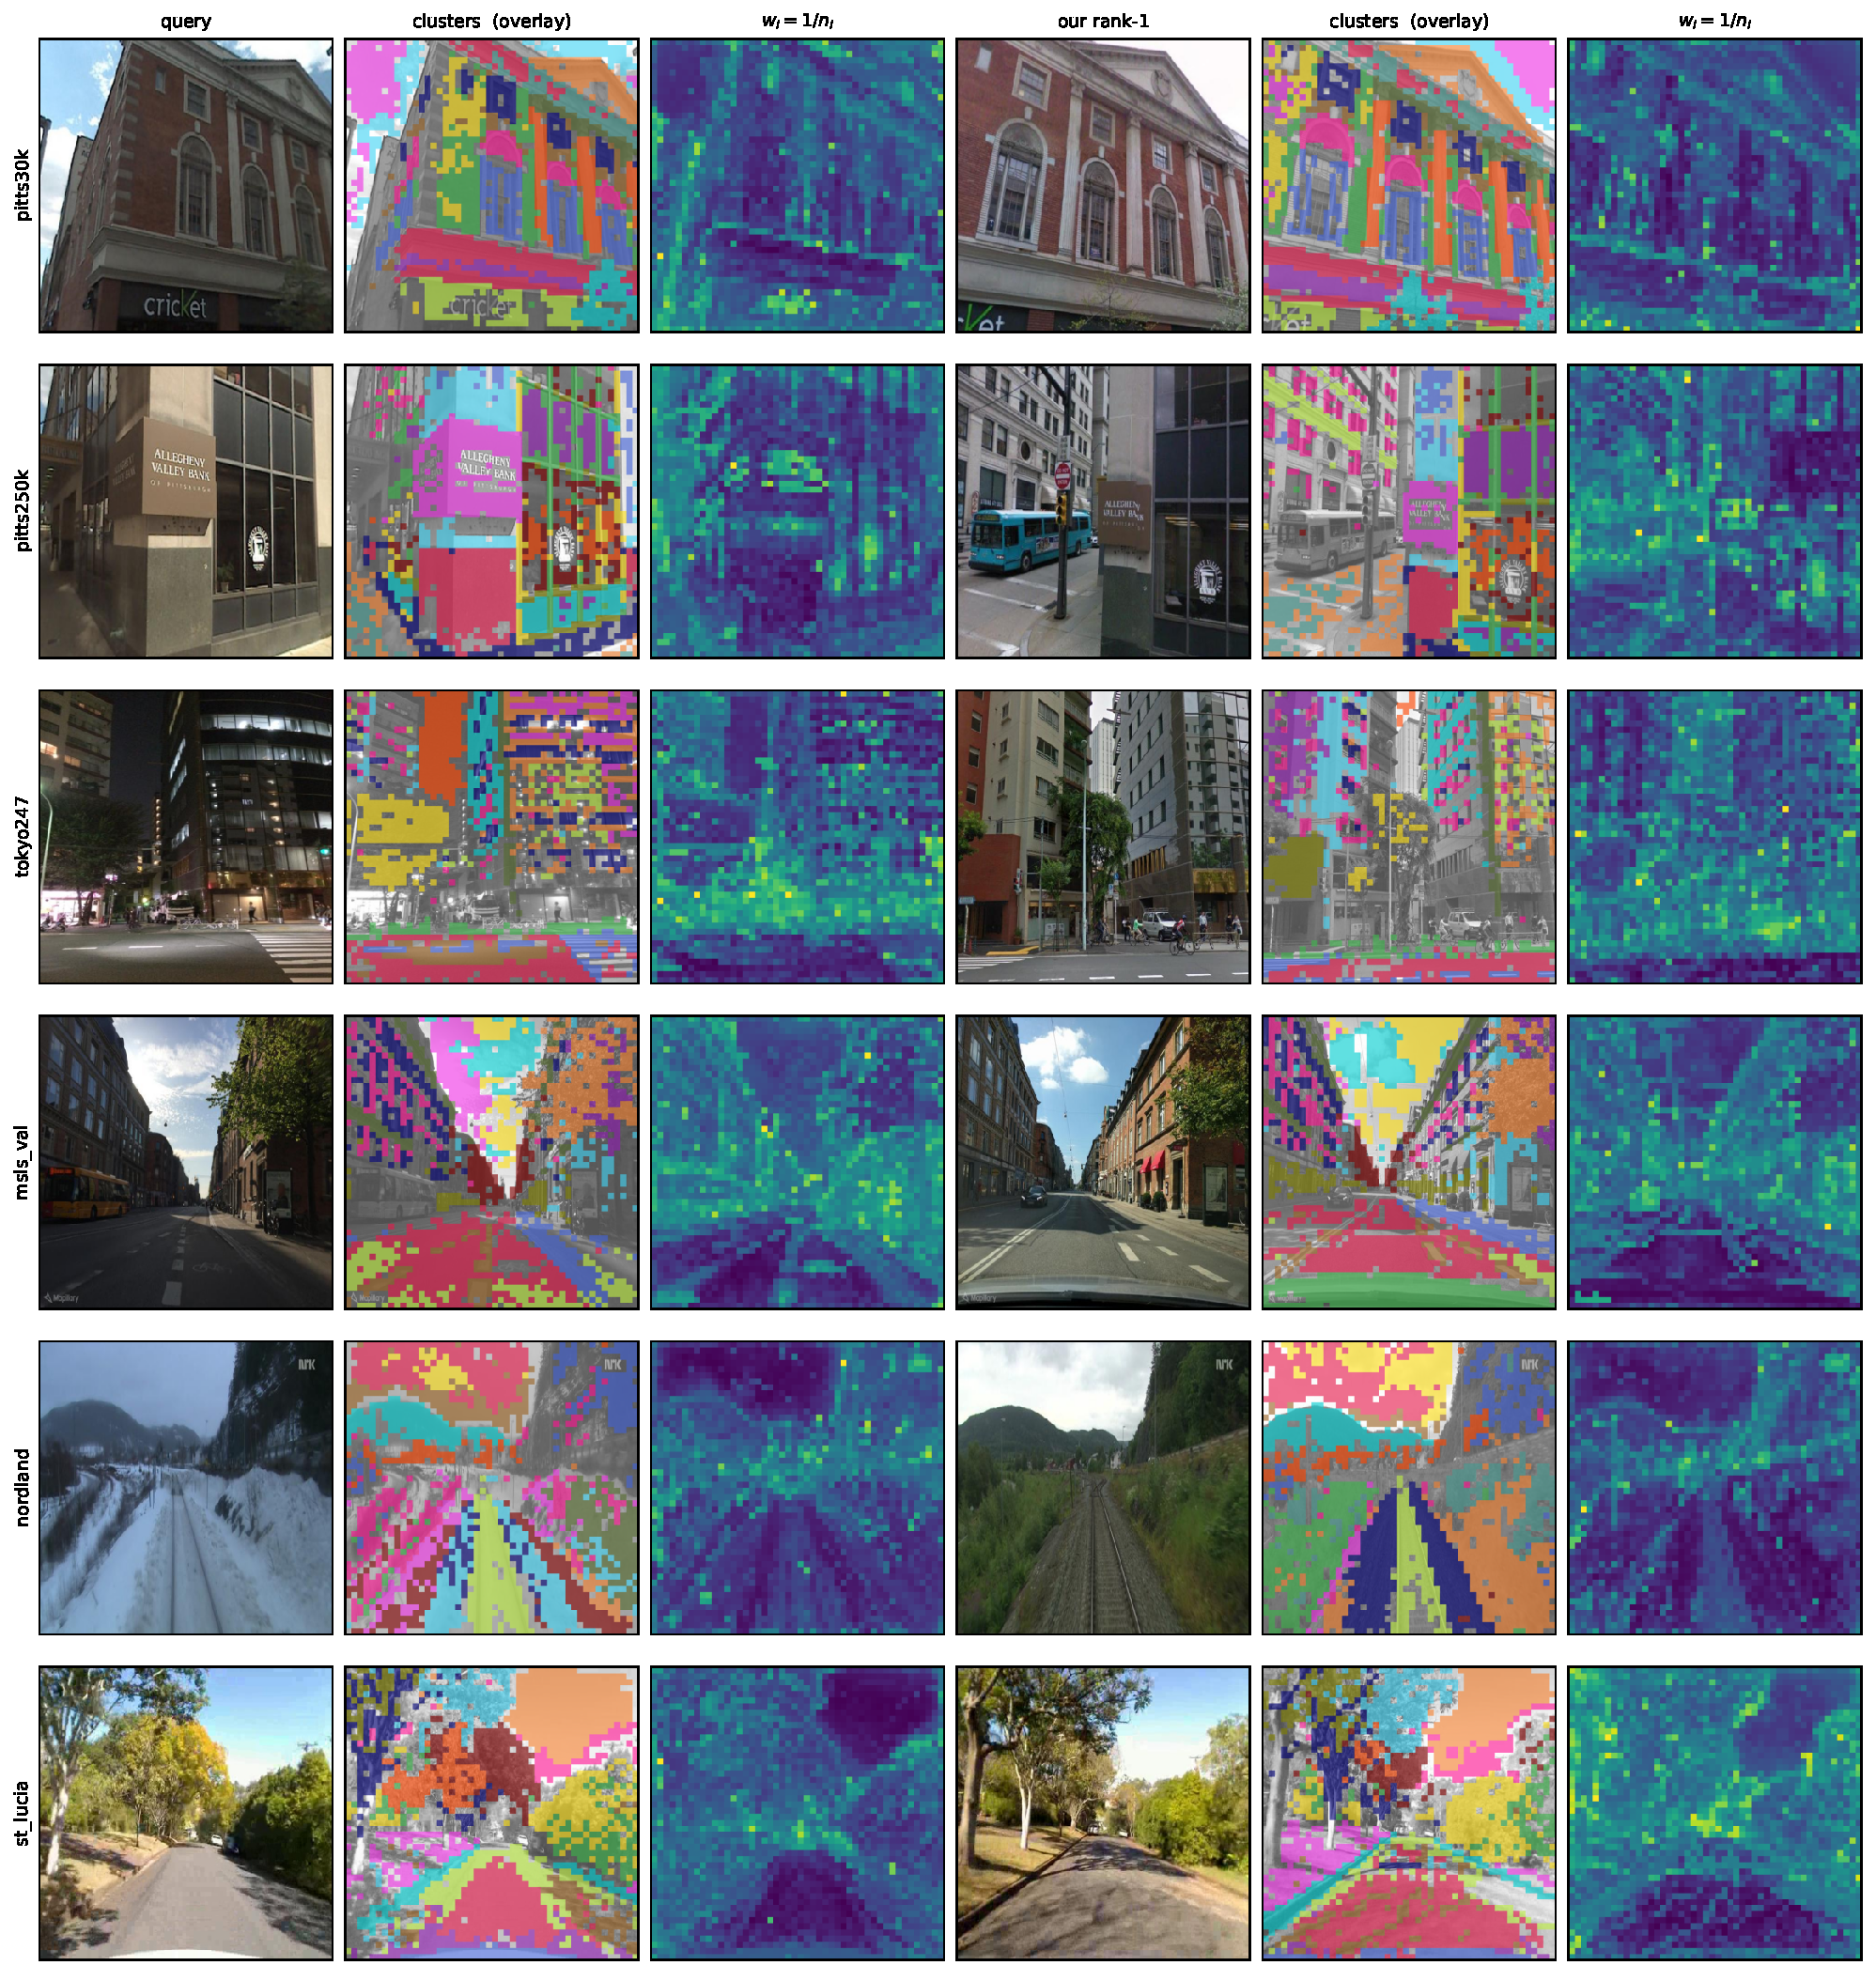
\includegraphics[width=\textwidth]{figures/all_clusters_1.pdf}
\caption{Near-duplicate blocks, benchmarks 1--6. Grey marks patches joining no block; the third and sixth columns show $w_i{=}1/n_i$ on a log scale over the full $2{,}304$ tokens.}
\label{fig:vis-c1}
\end{figure*}
\begin{figure*}[p]
\centering
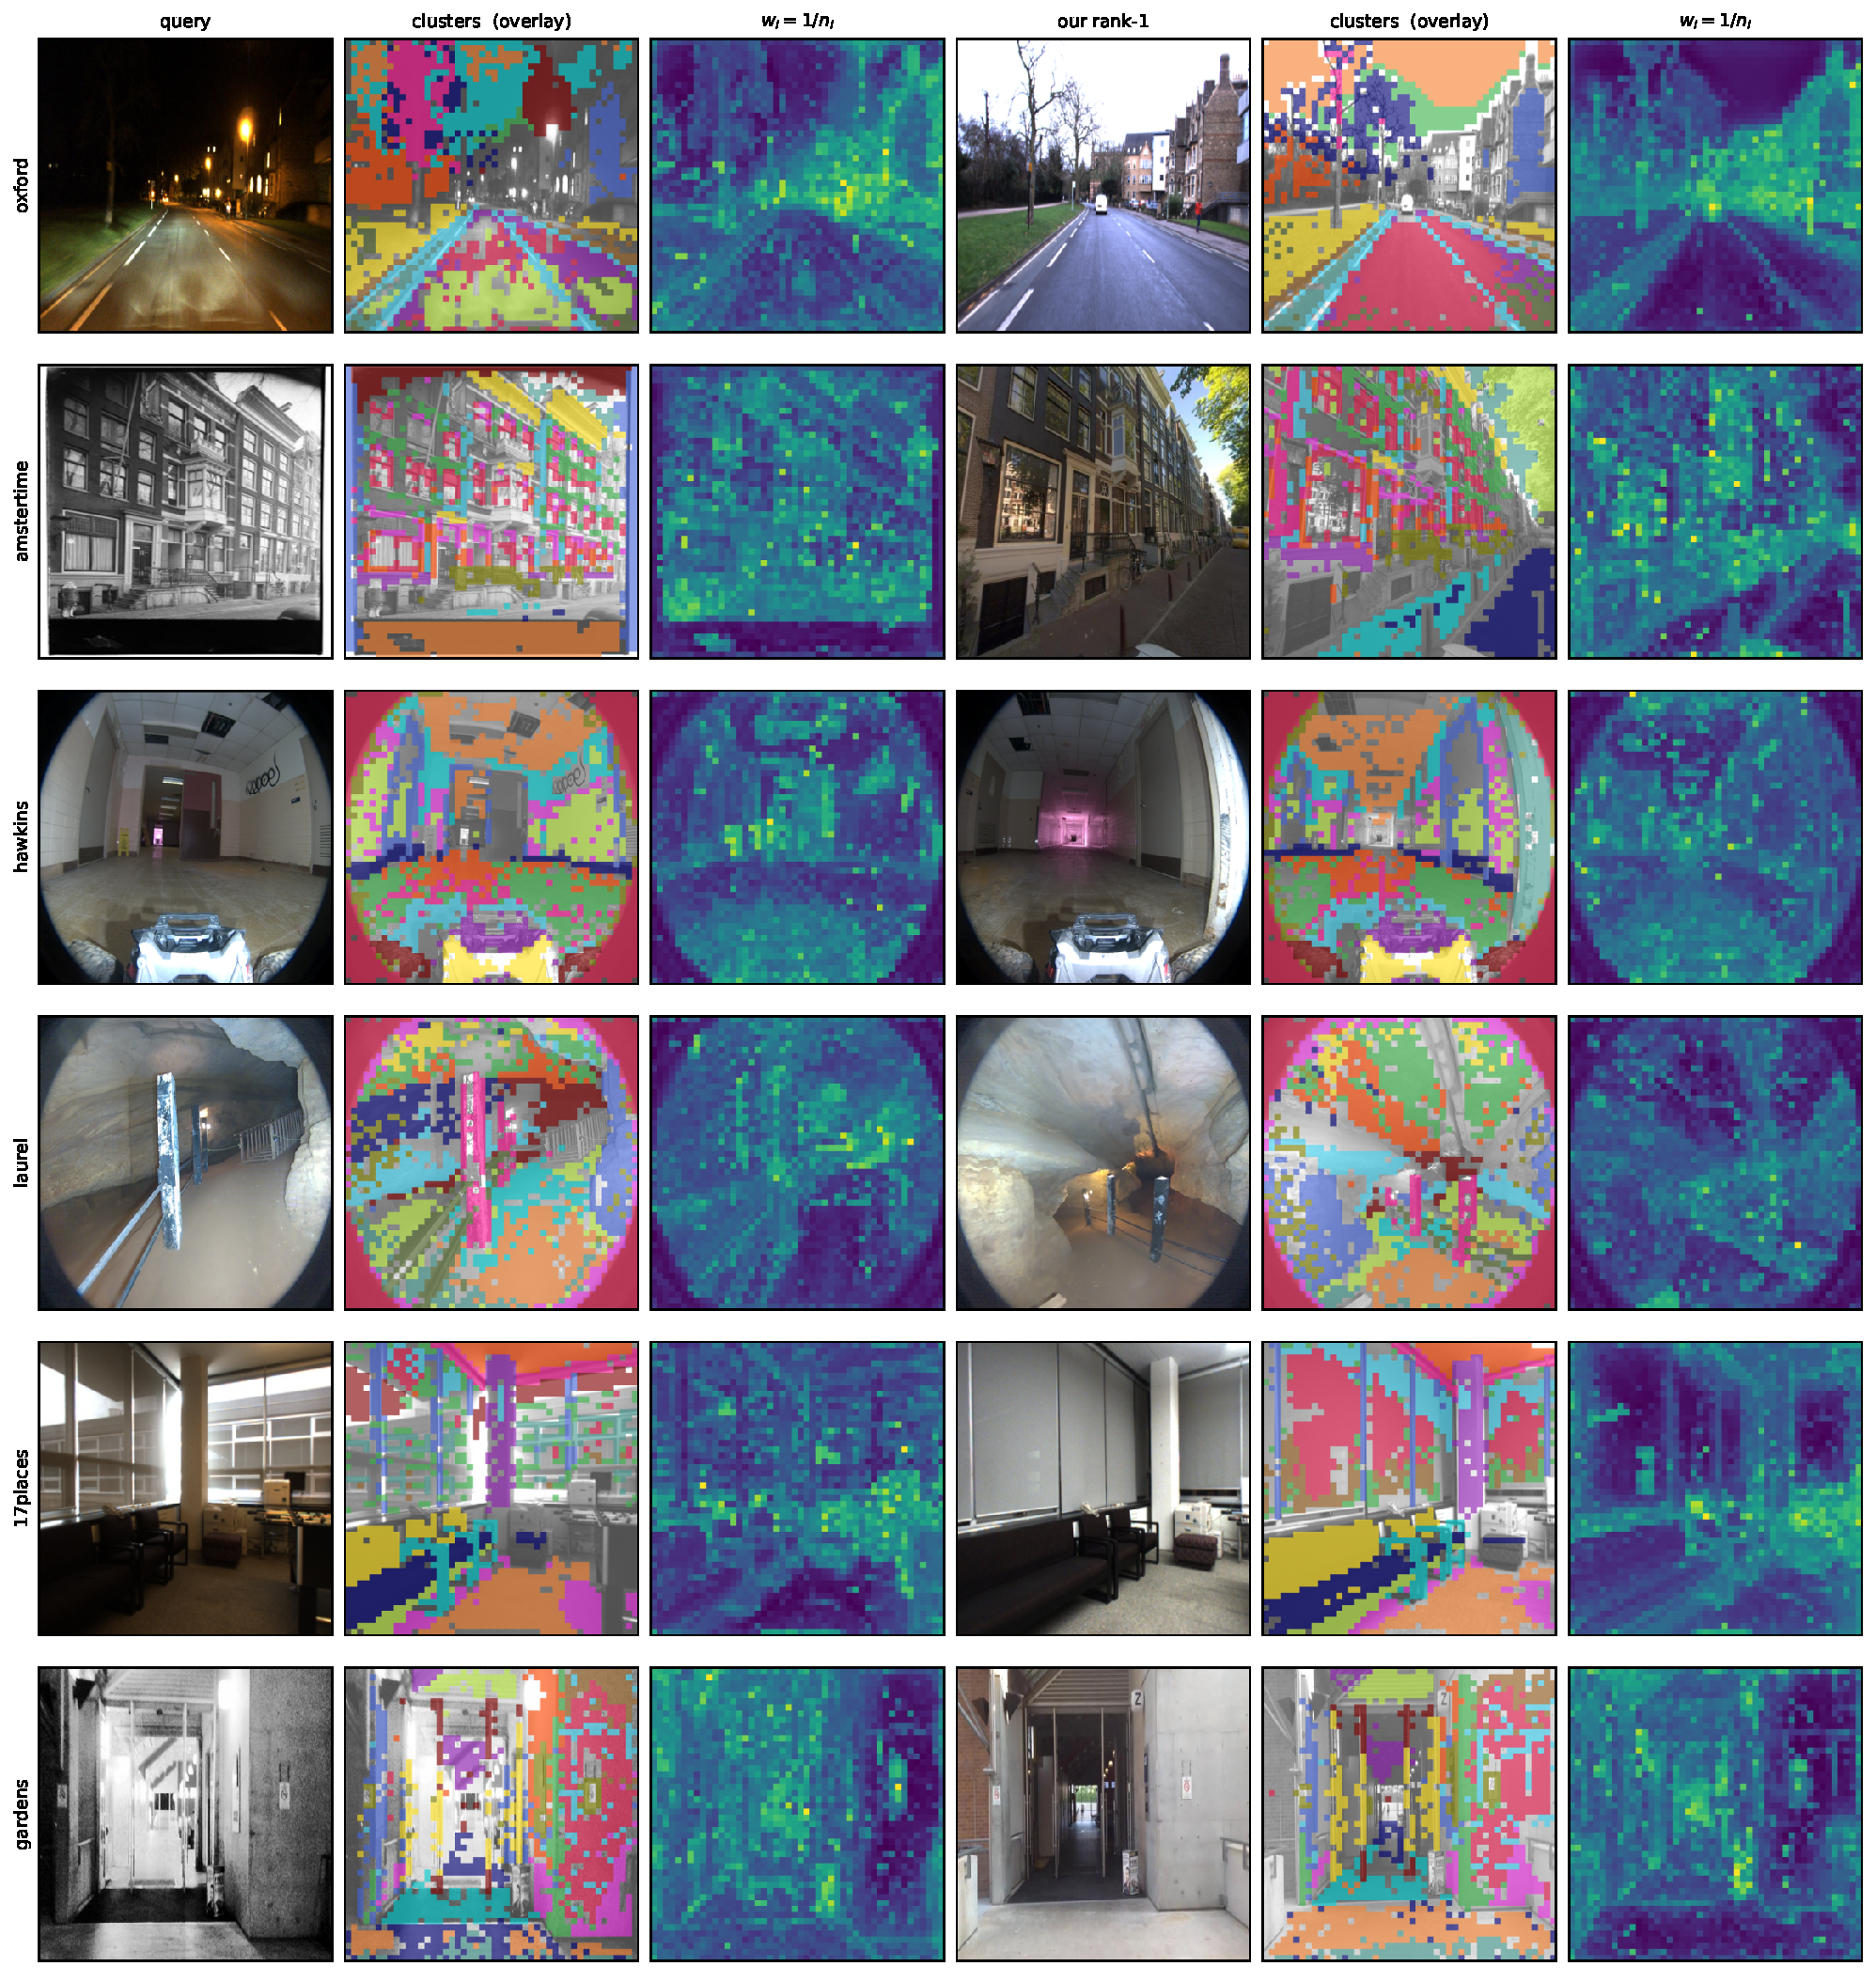
\includegraphics[width=\textwidth]{figures/all_clusters_2.pdf}
\caption{Near-duplicate blocks, benchmarks 7--12.}
\label{fig:vis-c2}
\end{figure*}
\begin{figure*}[p]
\centering
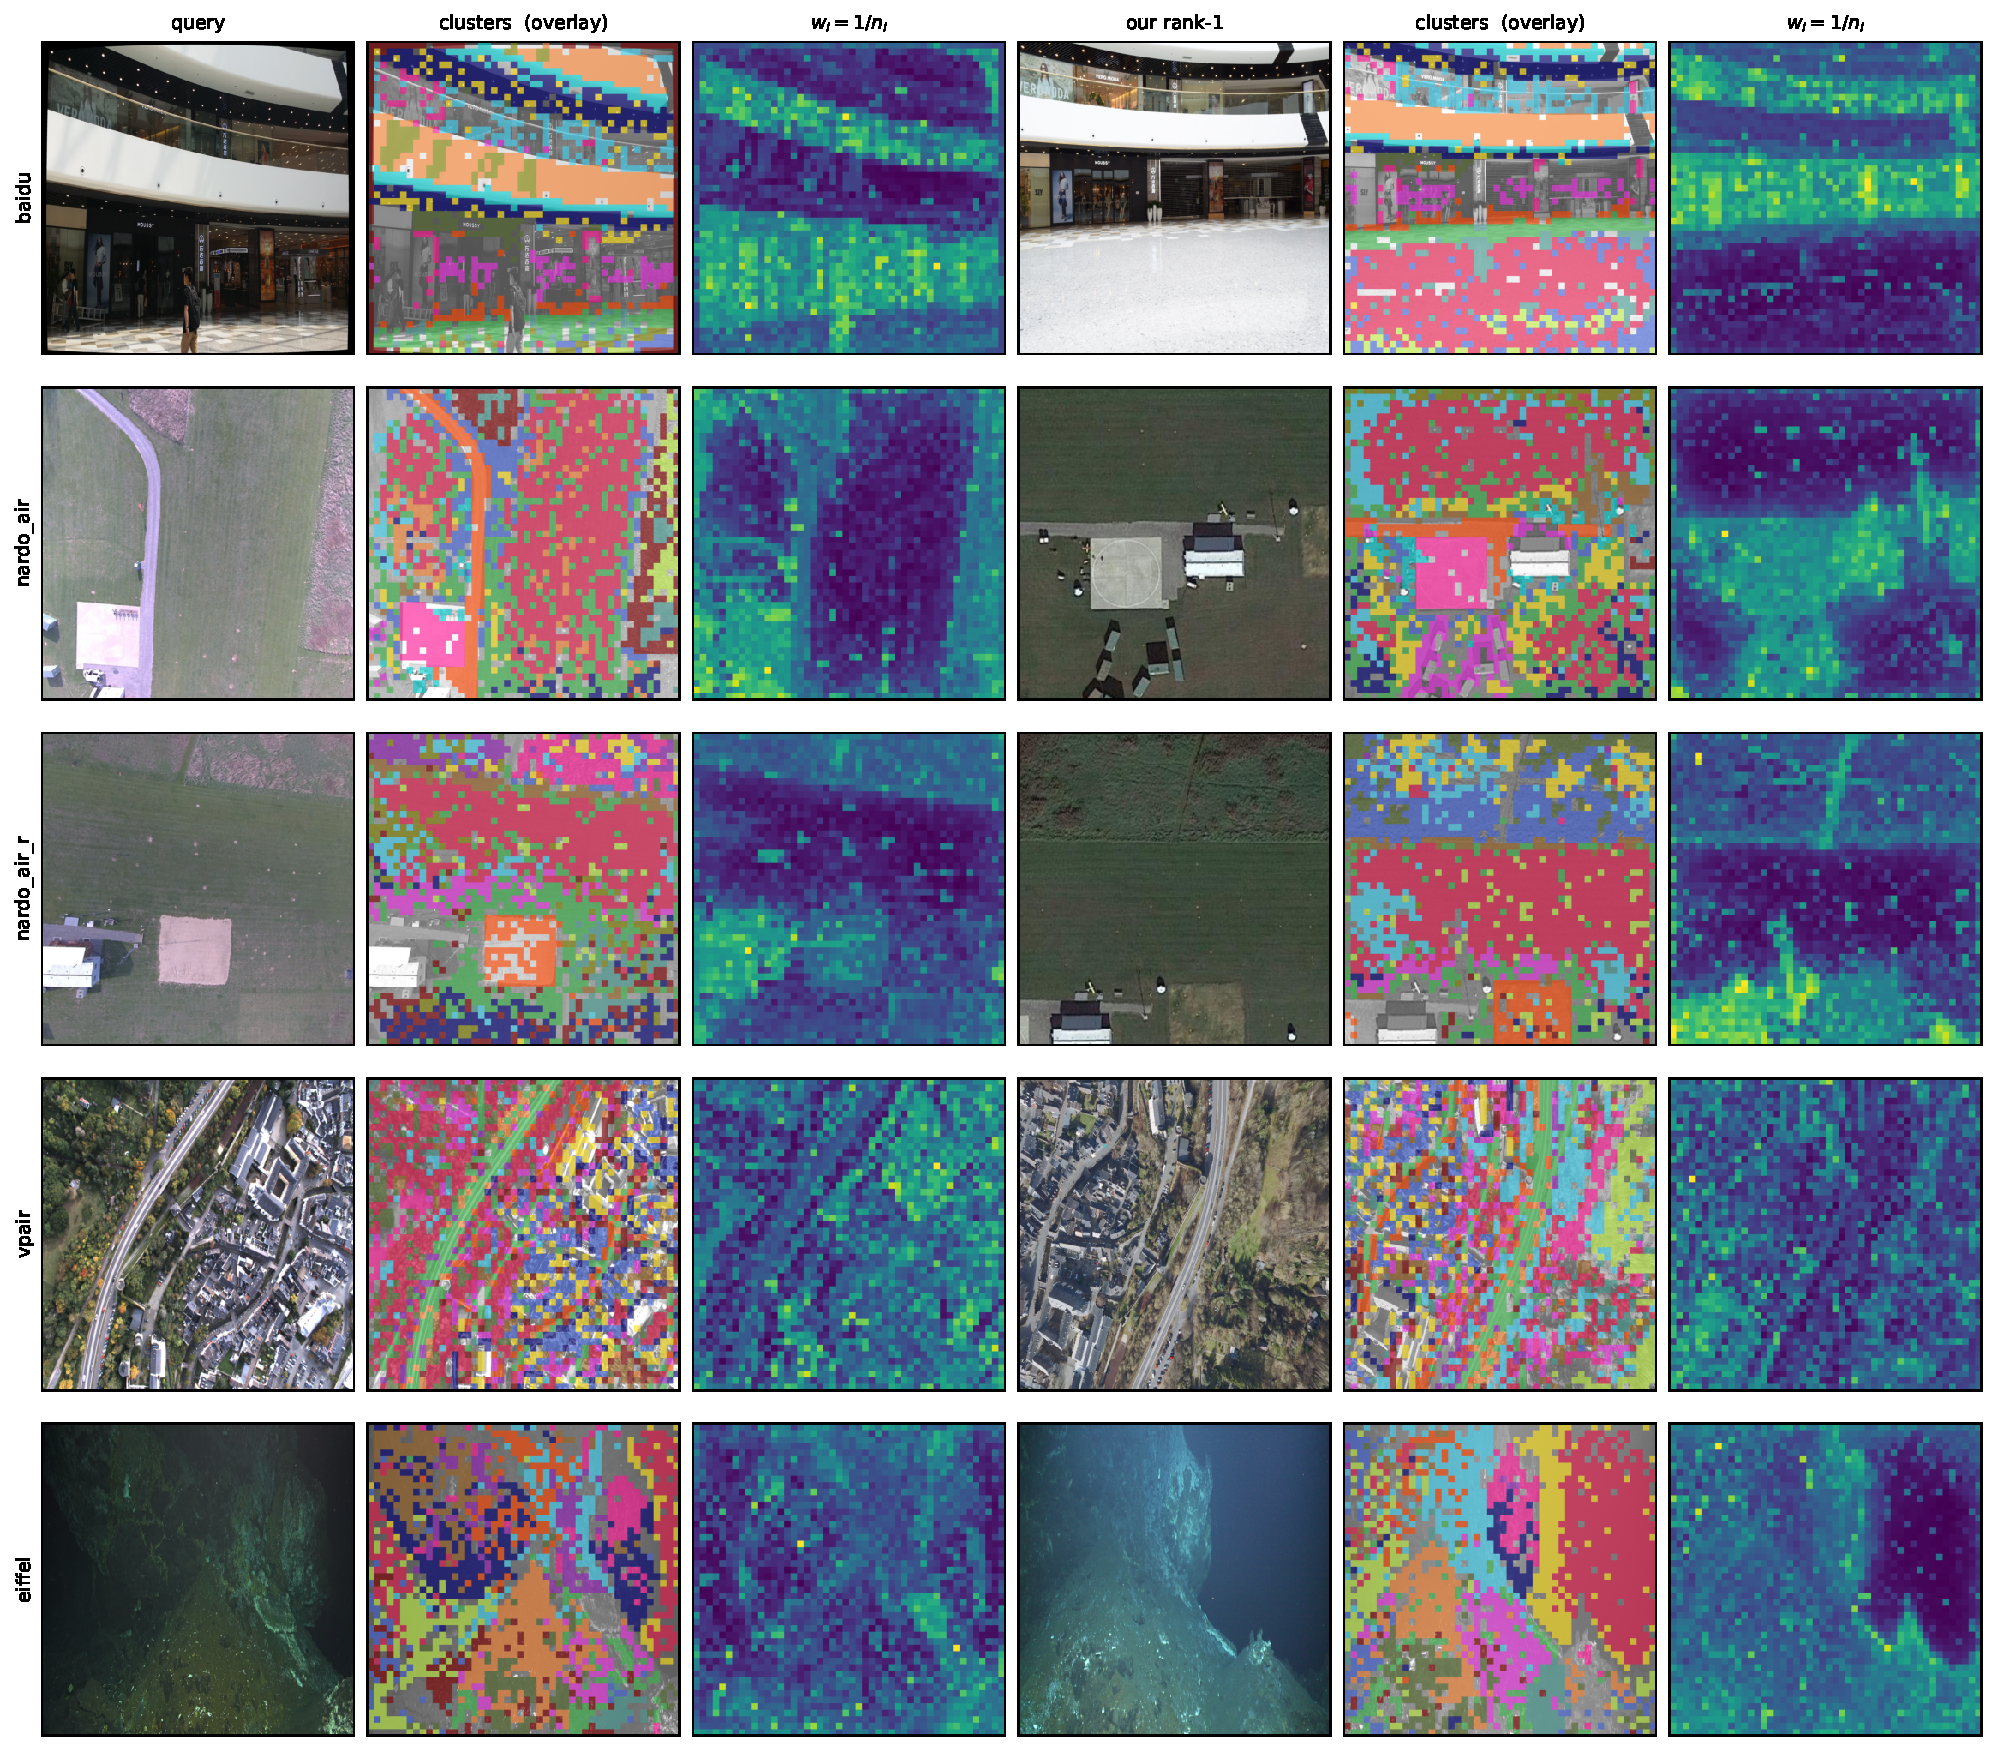
\includegraphics[width=\textwidth]{figures/all_clusters_3.pdf}
\caption{Near-duplicate blocks, benchmarks 13--17.}
\label{fig:vis-c3}
\end{figure*}

\section{The second-order descriptor}

\subsection{The coarse stage: factorial and reduction grid}
\label{sec:exp-stage1}
\label{sec:stage1abl}
\label{sec:compact}
\label{app:coarsegrid}
\begin{table}[t]
\caption{\textbf{Stage 1 alone on the nine environments.} R@1, single-stage global retrieval, every row our own run under one protocol at each method's native resolution. $^{\dagger}$reported after its own re-ranker; $^{o}$from our earlier operating point, as is the DINOv2-G row.}
\label{tab:coarse}
\begin{center}
{\scriptsize\setlength{\tabcolsep}{1.8pt}\renewcommand{\arraystretch}{0.86}%
\begin{tabular}{llccccccccc|c}
\toprule
& & Degr.\ & SubT & \multicolumn{3}{c}{Indoor} & \multicolumn{3}{c}{Aerial} & UW & \\
\cmidrule(lr){3-11}
Method   &   Backbone   &   Hawk   &   Laurel   &  17Pl &   Gard   &   Baidu   &   N-Air   &   N-AirR   &   VP-Air   & M-Atl &   mean \\
\midrule
\multicolumn{12}{l}{\emph{Trained / fine-tuned --- single-stage global descriptor}} \\
MegaLoc              &    DINOv2-B    &  37.3  &  55.4  &  64.8  &  95.5  &  \underline{79.4}  &  \textbf{85.9}  &  81.7  &  45.6  &  \textbf{40.6}  &  65.1\\
SAGE                 &    DINOv2-L    &  27.1  &  46.4  &  64.0  &  93.5  &  74.6  &  \textbf{85.9}  &  84.5  &  39.1  &  24.8  &  60.0\\
BoQ                  &    DINOv2-B    &  33.9  &  60.7  &  64.3  &  \underline{98.0}  &  77.4  &  62.0  &  91.5  &  29.5  &  35.6  &  61.4\\
CricaVPR             &    DINOv2-B    &  28.0  &  34.8  &  64.0  &  94.0  &  65.8  &  45.1  &  \textbf{100.0}  &  19.9  &  27.7  &  53.3\\
SALAD                &    DINOv2-B    &  38.1  &  46.4  &  64.3  &  96.5  &  69.9  &  53.5  &  94.4  &  24.0  &  15.8  &  55.9\\
CliqueMining         &    DINOv2-B    &  22.9  &  38.4  &  65.3  &  93.0  &  69.2  &  62.0  &  84.5  &  22.8  &  35.6  &  54.9\\
FoL$^{\dagger}$      & DINOv2-L       &  36.4  &  54.5  &  65.3  &  97.0  &  78.9  &  77.5  &  \underline{98.6}  &  46.7  &  25.7  &  64.5\\
EigenPlaces          &    R50         &  28.8  &  27.7  &  63.8  &  86.0  &  66.6  &  12.7  &  \textbf{100.0}  &  13.1  &  29.7  &  47.6\\
CosPlace             &    R50         &  33.9  &  25.9  &  63.3  &  84.5  &  47.1  &  0.0  &  76.1  &  10.4  &  32.7  &  41.5\\
SFRS                 &    VGG16       &  29.7  &  21.4  &  59.1  &  55.0  &  51.3  &  0.0  &  47.9  &  9.4  &  9.9  &  31.5\\
SelaVPR++$^{\dagger}$  &  DINOv2-L         &  21.2  &  35.7  &  65.0  &  95.5  &  73.6  &  81.7  &  87.3  &  42.7  &  27.7  &  58.9\\
Patch-NetVLAD        &    VGG16       &  39.0  &  59.8  &  63.1  &  74.5  &  66.8  &  63.4  &  71.8  &  16.0  &  23.8  &  53.1\\
R2Former$^{\dagger}$ & DeiT-S         &  17.8  &  30.4  &  63.8  &  84.0  &  74.7  &  26.8  &  83.1  &  15.0  &  22.8  &  46.5\\
VLAD-BuFF            &    DINOv2-B    &  37.3  &  33.9  &  64.5  &  96.5  &  76.4  &  57.8  &  88.7  &  33.3  &  27.7  &  57.4\\
SuperVLAD            &    DINOv2-B    &  37.3  &  51.8  &  64.8  &  95.5  &  70.3  &  14.1  &  88.7  &  23.8  &  13.9  &  51.1\\
SelaVPR$^{\dagger}$  & DINOv2-L       &  25.4  &  53.6  &  63.3  &  94.5  &  68.5  &  59.1  &  83.1  &  32.6  &  21.8  &  55.8\\
MixVPR               &    R50         &  26.3  &  32.1  &  63.8  &  92.0  &  68.4  &  39.4  &  78.9  &  12.9  &  24.8  &  48.7\\
NetVLAD              &    VGG16       &  38.1  &  42.9  &  63.8  &  66.0  &  57.8  &  9.9  &  39.4  &  14.7  &  26.7  &  39.9\\
\midrule
\multicolumn{12}{l}{\emph{Training-free --- frozen backbone, first-order pooling}} \\
GeM                  &    DINOv2-B    &  54.2  &  56.3  &  63.8  &  90.5  &  48.1  &  66.2  &  85.9  &  37.0  &  20.8  &  58.1\\
GeM                  &    DINOv2-L    &  55.9  &  56.3  &  63.8  &  92.5  &  46.4  &  \underline{80.3}  &  83.1  &  46.4  &  24.8  &  61.1\\
AnyLoc$^{p}$         &    DINOv2-G    &  \underline{65.2}  &  61.6  &  65.0  &  95.5  &  75.2  &  76.1  &  85.9  &  \underline{66.7}$^{d}$  &  34.6  &  \underline{69.5}\\
\midrule
\multicolumn{12}{l}{Ours \emph{--- training-free, second-order instance}} \\
Ours    &    DINOv2-B    &  58.5  &  60.7  &  63.6  &  94.0  &  71.7  &  47.9  &  84.5  &  43.0  &  35.6$^{o}$  &  62.2\\
Ours    &    DINOv2-L    &  \textbf{69.5}  &  50.9  &  64.0  &  96.0  &  73.8  &  36.6  &  84.5  &  49.5  &  \underline{36.6}$^{o}$  &  62.4\\
Ours    &    DINOv2-G    &  56.8  &  \underline{67.9}  &  65.0  &  96.5  &  76.7  &  74.7  &  95.8  &  48.2  &  35.6  &  68.6\\
Ours    &    DINOv3-L    &  59.3  &  \textbf{69.6}  &  64.3  &  95.0  &  78.2  &  42.3  &  87.3  &  56.0  &  31.7$^{o}$  &  64.9\\
Ours    &    DINOv3-7B    &  52.5  &  60.7  &  \underline{65.5}  &  95.5  &  77.2  &  74.7  &  95.8  &  \textbf{73.4}  &  34.7$^{o}$  &  \textbf{70.0}\\
\bottomrule
\end{tabular}%
}
\end{center}
\end{table}
\begin{table}[t]
\caption{\textbf{The instance-and-device factorial at a matched $1024$-d budget} (compressed before scoring). Uncompressed, the second order leads all six statistics; at this budget the orders trade domains, and the weight remains the largest device in both ($7.0$ and $18.7$ mean R@1).}
\label{tab:firstsecond}
\begin{center}
{\scriptsize\setlength{\tabcolsep}{2.2pt}%
\resizebox{\textwidth}{!}{%
\begin{tabular}{lccccccc|c}
\toprule
 & \multicolumn{7}{c}{per database} & \multicolumn{1}{c}{summary$^\dagger$} \\
\cmidrule(lr){2-8}\cmidrule(lr){9-9}
Configuration   &   Amst   &   SF$^\ast$   &   Pitts   &   VP-Air   &   MSLS   &   Nord   &   Tokyo   &   mean \\
    &  \tiny 1.2k &  \tiny 8.0k &  \tiny 10k &  \tiny 12.7k &  \tiny 18.9k &  \tiny 27.6k &  \tiny 76.0k & \\
\midrule \multicolumn{9}{l}{\emph{\textbf{R@1}} \ \ \scriptsize mean over the $6$ databases both orders share} \\
\multicolumn{9}{l}{\ \ First order (VLAD)} \\
\ \ \ none    &  26.16 &  52.67 &  74.94 &  44.09 &  34.46 &  10.89 &  68.89 &  40.54 \\
\ \ \ intra-norm    &  46.55 &  68.07 &  85.62 &  55.99 &  53.38 &  12.94 &  91.11 &  53.76 \\
\ \ \ power law    &  40.70 &  63.20 &  80.34 &  46.27 &  42.16 &  16.21 &  80.95 &  48.15 \\
\ \ \ intra-norm $+$ power law    &  47.77 &  68.85 &  85.18 &  52.73 &  52.03 &  15.92 &  88.89 &  53.75 \\
\ \ \ $w$    &  34.69 &  76.06 &  84.30 &  43.02 &  65.00 &  35.54 &  54.29 &  56.44 \\
\ \ \ $w$ $+$ intra-norm    &  46.95 &  63.94 &  85.14 &  52.18 &  51.22 &  15.13 &  88.57 &  52.43 \\
\ \ \ $w$ $+$ intra-norm $+$ power law    &  47.12 &  65.24 &  84.32 &  50.70 &  50.14 &  17.27 &  85.71 &  52.46 \\
\ \ \ \textbf{$w$ $+$ power law}    &  45.57 &  80.42 &  86.38 &  48.60 &  70.41 &  44.82 &  78.73 &  62.70 \\
\multicolumn{9}{l}{\ \ Second order (covariance)} \\
\ \ \ none    &  21.85 &  38.67 &  72.84 &  37.14 &  24.86 &  4.90 &    ---    &  33.38 \\
\ \ \ spectral $\alpha{=}\tfrac12$    &  34.12 &  54.68 &  80.55 &  40.06 &  36.89 &  10.93 &    ---    &  42.87 \\
\ \ \ power law    &  33.79 &  52.99 &  77.14 &  38.54 &  33.65 &  15.19 &    ---    &  41.88 \\
\ \ \ spectral $+$ power law    &  41.27 &  64.44 &  81.94 &  35.66 &  44.32 &  23.33 &    ---    &  48.49 \\
\ \ \ $w$    &  42.32 &  75.06 &  87.05 &  42.13 &  69.19 &  35.21 &    ---    &  58.49 \\
\ \ \ $w$ $+$ spectral    &  45.90 &  75.26 &  88.12 &  44.68 &  68.92 &  39.63 &    ---    &  60.42 \\
\ \ \ $w$ $+$ spectral $+$ power law    &  46.71 &  73.61 &  88.04 &  38.06 &  67.84 &  51.19 &    ---    &  60.91 \\
\ \ \ \textbf{$w$ $+$ power law}    &  45.49 &  74.46 &  87.40 &  43.83 &  68.11 &  51.39 &    ---    &  61.78 \\
\midrule \multicolumn{9}{l}{\emph{\textbf{R@100}} \ \ \scriptsize mean over the $6$ databases both orders share} \\
\multicolumn{9}{l}{\ \ First order (VLAD)} \\
\ \ \ none    &  79.45 &  83.87 &  95.25 &  79.34 &  62.84 &  39.58 &  96.19 &  73.39 \\
\ \ \ intra-norm    &  93.58 &  95.99 &  99.16 &  90.28 &  86.89 &  51.10 &  98.73 &  86.17 \\
\ \ \ power law    &  91.71 &  93.80 &  97.29 &  83.07 &  78.24 &  51.98 &  98.73 &  82.68 \\
\ \ \ intra-norm $+$ power law    &  94.48 &  96.42 &  99.11 &  88.40 &  85.54 &  54.32 &  98.41 &  86.38 \\
\ \ \ $w$    &  90.33 &  97.80 &  98.93 &  90.84 &  92.57 &  81.13 &  92.06 &  91.93 \\
\ \ \ $w$ $+$ intra-norm    &  93.99 &  95.59 &  99.18 &  92.76 &  87.57 &  53.75 &  98.10 &  87.14 \\
\ \ \ $w$ $+$ intra-norm $+$ power law    &  94.23 &  96.22 &  98.99 &  90.24 &  85.81 &  55.19 &  98.10 &  86.78 \\
\ \ \ \textbf{$w$ $+$ power law}    &  94.48 &  98.18 &  99.16 &  89.06 &  95.14 &  82.27 &  97.14 &  93.05 \\
\multicolumn{9}{l}{\ \ Second order (covariance)} \\
\ \ \ none    &  71.32 &  69.26 &  93.79 &  71.91 &  53.92 &  24.28 &    ---    &  64.08 \\
\ \ \ spectral $\alpha{=}\tfrac12$    &  87.00 &  87.71 &  96.96 &  72.84 &  71.62 &  40.56 &    ---    &  76.11 \\
\ \ \ power law    &  88.87 &  87.86 &  96.13 &  74.32 &  67.70 &  47.43 &    ---    &  77.05 \\
\ \ \ spectral $+$ power law    &  91.96 &  94.23 &  97.48 &  68.96 &  77.84 &  59.82 &    ---    &  81.72 \\
\ \ \ $w$    &  92.36 &  96.73 &  99.19 &  84.29 &  94.32 &  77.41 &    ---    &  90.72 \\
\ \ \ $w$ $+$ spectral    &  93.34 &  96.78 &  99.33 &  82.22 &  93.65 &  77.82 &    ---    &  90.52 \\
\ \ \ $w$ $+$ spectral $+$ power law    &  93.99 &  96.72 &  99.35 &  76.09 &  93.24 &  84.06 &    ---    &  90.58 \\
\ \ \ \textbf{$w$ $+$ power law}    &  93.74 &  97.03 &  99.24 &  85.03 &  94.19 &  85.63 &    ---    &  92.48 \\
\midrule \multicolumn{9}{l}{\emph{\textbf{R@1000}} \ \ \scriptsize mean over the $4$ databases both orders share; AmsterTime and SF-XL val are shown but excluded from the summary, where a top-$1000$ list is $81\%$ and $12.5\%$ of the database} \\
\multicolumn{9}{l}{\ \ First order (VLAD)} \\
\ \ \ none    &  99.43 &  98.70 &  99.87 &  96.05 &  87.97 &  76.66 &  \textbf{100.00} &  90.14 \\
\ \ \ intra-norm    &  \textbf{100.00} &  99.84 &  \textbf{100.00} &  \textbf{99.78} &  97.70 &  81.03 &  \textbf{100.00} &  94.63 \\
\ \ \ power law    &  99.84 &  99.84 &  \textbf{100.00} &  98.45 &  96.49 &  83.37 &  \underline{99.68} &  94.58 \\
\ \ \ intra-norm $+$ power law    &  \textbf{100.00} &  \textbf{99.91} &  \textbf{100.00} &  \textbf{99.78} &  98.11 &  83.06 &  \underline{99.68} &  95.24 \\
\ \ \ $w$    &  99.84 &  99.87 &  \textbf{100.00} &  99.70 &  98.11 &  \underline{97.19} &  99.05 &  98.75 \\
\ \ \ $w$ $+$ intra-norm    &  \textbf{100.00} &  99.80 &  \textbf{100.00} &  \underline{99.74} &  98.11 &  81.53 &  \underline{99.68} &  94.84 \\
\ \ \ $w$ $+$ intra-norm $+$ power law    &  \textbf{100.00} &  99.86 &  \textbf{100.00} &  \underline{99.74} &  98.11 &  83.51 &  99.05 &  95.34 \\
\ \ \ \textbf{$w$ $+$ power law}    &  \textbf{100.00} &  \underline{99.90} &  \textbf{100.00} &  \textbf{99.78} &  \textbf{99.05} &  97.03 &  \underline{99.68} &  \underline{98.97} \\
\multicolumn{9}{l}{\ \ Second order (covariance)} \\
\ \ \ none    &  99.76 &  90.81 &  \underline{99.88} &  94.09 &  77.70 &  60.02 &    ---    &  82.92 \\
\ \ \ spectral $\alpha{=}\tfrac12$    &  \underline{99.92} &  98.91 &  \textbf{100.00} &  95.45 &  90.00 &  75.87 &    ---    &  90.33 \\
\ \ \ power law    &  \underline{99.92} &  99.36 &  \textbf{100.00} &  93.31 &  90.54 &  82.27 &    ---    &  91.53 \\
\ \ \ spectral $+$ power law    &  \textbf{100.00} &  99.76 &  \textbf{100.00} &  94.38 &  96.22 &  86.25 &    ---    &  94.21 \\
\ \ \ $w$    &  \textbf{100.00} &  99.85 &  \textbf{100.00} &  99.19 &  98.24 &  94.32 &    ---    &  97.94 \\
\ \ \ $w$ $+$ spectral    &  \textbf{100.00} &  99.89 &  \textbf{100.00} &  98.97 &  \underline{98.38} &  94.30 &    ---    &  97.91 \\
\ \ \ $w$ $+$ spectral $+$ power law    &  \textbf{100.00} &  99.87 &  \textbf{100.00} &  99.26 &  98.24 &  96.84 &    ---    &  98.59 \\
\ \ \ \textbf{$w$ $+$ power law}    &  \textbf{100.00} &  99.84 &  \textbf{100.00} &  99.67 &  98.24 &  \textbf{98.12} &    ---    &  \textbf{99.01} \\
\bottomrule
\end{tabular}%
}%
}
\end{center}
\end{table}
\begin{table}[t]
\caption{\textbf{Token pruning $\times$ whitened compression, single-stage coarse retrieval} (R@1; five test benchmarks and their mean). Both orders, both backbones, one protocol; keep-$N$ selects by $w_i$ computed on the full token set. $^\dagger$AmsterTime rank-caps the WPCA below $2{,}048$-d; its $1{,}024$-d value shown. R@1000 never falls below $98.4$ (7B) / $96.3$ (L) anywhere in the grid.}
\label{tab:prunecomp}
\begin{center}
\scriptsize
\setlength{\tabcolsep}{3.4pt}
\renewcommand{\arraystretch}{1.02}
\resizebox{\textwidth}{!}{%
\begin{tabular}{lll rrrrr r rrrrr r}
\toprule
& & & \multicolumn{6}{c}{DINOv3-7B} & \multicolumn{6}{c}{DINOv3-L} \\
\cmidrule(lr){4-9}\cmidrule(lr){10-15}
Order   &   keep   &   compression   &   Pitts   &   MSLS   &   Nord   &   Tokyo   &   Amst   &   mean   &   Pitts   &   MSLS   &   Nord   &   Tokyo   &   Amst   &   mean \\
\midrule
2nd   &   full    &   raw              &  88.51 &  70.95 &  63.98 &  93.02 &  51.58 &  73.61 &  88.97 &  69.73 &  43.82 &  91.75 &  44.27 &  67.71\\
       &             &    WPCA-1024         &  89.61 &  83.78 &  60.14 &  93.65 &  67.67 &  78.97 &  89.67 &  82.57 &  37.47 &  90.48 &  61.49 &  72.34\\
       &             &    WPCA-2048         &  89.80 &  86.49 &  62.18 &  95.87 &  67.67$^\dagger$ &  80.40 &  89.57 &  84.19 &  42.19 &  92.38 &  61.49$^\dagger$ &  73.96\\
\addlinespace[2pt]
2nd   &   1024    &   raw              &  89.22 &  74.32 &  69.33 &  92.06 &  48.09 &  74.60 &  89.10 &  73.65 &  44.31 &  87.30 &  40.29 &  66.93\\
       &             &    WPCA-1024         &  90.45 &  84.86 &  70.78 &  92.70 &  66.04 &  80.97 &  89.99 &  84.05 &  43.98 &  86.67 &  59.55 &  72.85\\
       &             &    \textbf{WPCA-2048}    &  91.02 &  86.89 &  75.09 &  94.92 &  66.04$^\dagger$ &  82.79 &  90.64 &  84.19 &  49.75 &  90.79 &  59.55$^\dagger$ &  74.98\\
\addlinespace[2pt]
2nd   &   512     &   raw              &  87.71 &  74.05 &  71.17 &  85.40 &  40.62 &  71.79 &  87.29 &  72.43 &  43.58 &  81.90 &  33.23 &  63.69\\
       &             &    WPCA-1024         &  90.40 &  84.19 &  74.26 &  89.52 &  60.52 &  79.78 &  89.50 &  84.05 &  48.66 &  83.49 &  51.18 &  71.38\\
       &             &    WPCA-2048         &  91.07 &  86.76 &  78.06 &  93.33 &  60.52$^\dagger$ &  81.95 &  90.60 &  82.97 &  53.81 &  89.21 &  51.18$^\dagger$ &  73.55\\
\midrule
1st   &   full    &   raw              &  86.52 &  71.22 &  67.41 &  92.70 &  52.40 &  74.05 &  86.84 &  67.16 &  40.27 &  90.48 &  45.90 &  66.13\\
       &             &    WPCA-1024         &  87.32 &  84.05 &  56.07 &  94.29 &  62.47 &  76.84 &  87.24 &  77.70 &  30.26 &  92.70 &  55.89 &  68.76\\
       &             &    WPCA-2048         &  87.21 &  83.24 &  54.37 &  95.56 &  62.47$^\dagger$ &  76.57 &  86.75 &  79.59 &  30.07 &  91.11 &  55.89$^\dagger$ &  68.68\\
\addlinespace[2pt]
1st   &   1024    &   raw              &  87.62 &  77.03 &  79.56 &  89.84 &  51.26 &  77.06 &  87.28 &  72.30 &  49.61 &  87.30 &  44.11 &  68.12\\
       &             &    WPCA-1024         &  88.47 &  85.00 &  61.48 &  92.06 &  60.03 &  77.41 &  88.15 &  81.62 &  34.48 &  88.89 &  53.05 &  69.24\\
       &             &    WPCA-2048         &  88.98 &  85.00 &  59.55 &  95.56 &  60.03$^\dagger$ &  77.82 &  88.50 &  80.68 &  35.13 &  89.52 &  53.05$^\dagger$ &  69.38\\
\addlinespace[2pt]
1st   &   512     &   raw              &  85.52 &  77.70 &  79.54 &  81.59 &  44.60 &  73.79 &  86.15 &  71.89 &  49.62 &  80.95 &  37.69 &  65.26\\
       &             &    WPCA-1024         &  87.57 &  84.32 &  61.93 &  85.08 &  51.42 &  74.06 &  86.83 &  79.46 &  35.88 &  79.37 &  43.54 &  65.02\\
       &             &    WPCA-2048         &  87.60 &  83.92 &  58.96 &  87.94 &  51.42$^\dagger$ &  73.97 &  87.50 &  79.73 &  36.78 &  81.59 &  43.54$^\dagger$ &  65.83\\
\bottomrule
\end{tabular}}
\end{center}
\end{table}

\subsection{What the weight does to the descriptor}
\label{app:patchvis-main}
\begin{figure}[H]
\centering
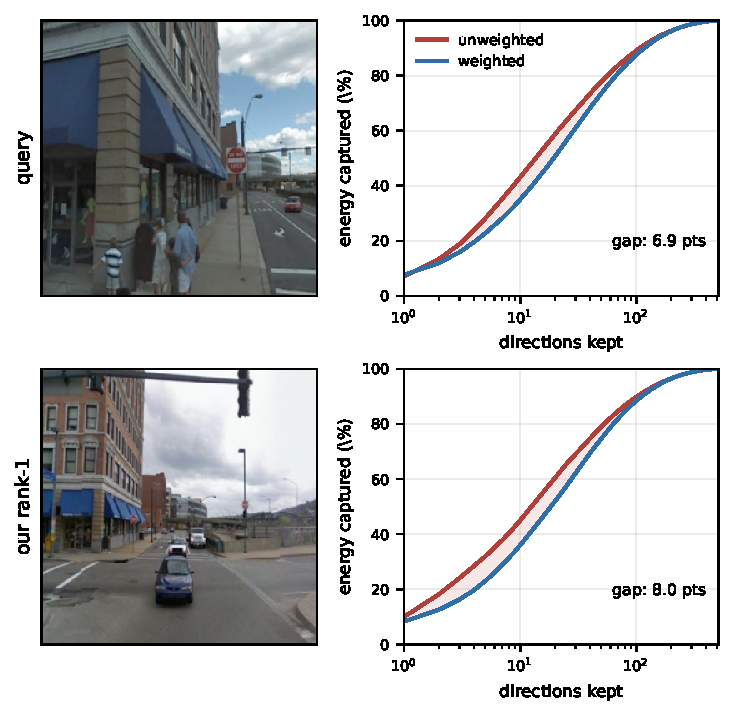
\includegraphics[width=0.50\textwidth]{figures/patch_cov.pdf}
\caption{\textbf{What the weight does to the descriptor.} One query and the database image our first stage retrieves for it. The right column reads $F^{\top}F$ and $G_C{=}F^{\top}WF$ as a distribution of the image's energy over directions: keeping the $k$ strongest directions captures the plotted share of the total, so a curve that rises early is one where a few directions carry the image. An element covering much of the frame arrives as many near-identical patches pointing the same way and concentrates the unweighted moment; the weight spreads it back, by $6.9$ and $8.0$ points averaged over the first $32$ directions.}
\label{fig:patchcov}
\end{figure}

\section{\textsc{MaxSim} re-ranking}

\subsection{Token budget against re-ranking operator}
\label{app:s2grid}
\begin{table}[h]
\caption{\textbf{Seven re-ranking operators $\times$ two token budgets}, mean R@1 over the nine environment sets of Table~\ref{tab:ood}. The coarse stage is the deployed one throughout; only the second stage changes. \textsc{selfw\_conf} is \eqref{eq:stage2}, the operator we adopt.}
\label{tab:s2grid}
\begin{center}
{\footnotesize\setlength{\tabcolsep}{3pt}%
\begin{tabular}{llccccccc}
\toprule
Backbone & tokens & base & \textsc{selfw} & \textsc{conf} & \textsc{selfw\_conf} & \textsc{mnn} & \textsc{mnn\_selfw} & comb. \\
\midrule
DINOv3-L  & keep-$1024$ & \textbf{74.85} & 74.07 & 73.89 & 73.56 & 71.10 & 70.74 & 70.50 \\
DINOv3-L  & all $2{,}304$ & 72.56 & 74.13 & 72.43 & \textbf{75.42} & 70.15 & 71.48 & 70.81 \\
\addlinespace[2pt]
DINOv3-7B & keep-$1024$ & 75.27 & 75.41 & 74.50 & \textbf{76.30} & 74.34 & 70.72 & 70.56 \\
DINOv3-7B & all $2{,}304$ & 71.68 & 74.90 & 69.04 & \textbf{76.57} & 70.46 & 72.10 & 71.63 \\
\bottomrule
\end{tabular}%
}
\end{center}
\end{table}

\subsection{Against \textsc{EffoVPR}'s criterion at a matched stage 1}
\label{app:effo-matched}
\begin{table}[t]
\caption{\textbf{Scoring rules at a matched stage 1} (Pitts30k, R@1; shortlist and features identical). \emph{lift} is over the class-token retrieval that produced the shortlist. $T_1$ is \textsc{EffoVPR}'s attention threshold, reported at the keypoint budget it induces.}
\label{tab:effo-matched}
\begin{center}
{\small
\begin{tabular}{lcc}
\toprule
Stage 2 & R@1 & lift \\
\midrule
none (class-token retrieval) & 77.93 & --- \\
\midrule
\multicolumn{3}{l}{\emph{Selection by attention} (\textsc{EffoVPR})} \\
keep all, mutual NN & 87.82 & $+9.89$ \\
$T_1$ at $512$ keypoints & \underline{88.70} & $+10.77$ \\
$T_1$ at $256$ & 86.66 & $+8.73$ \\
$T_1$ at $130$ & 82.51 & $+4.58$ \\
$T_1$ at $65$ & 77.93 & $+0.00$ \\
\midrule
\multicolumn{3}{l}{\emph{Weighting by self-similarity} (ours)} \\
\textsc{MaxSim}, unweighted & 86.53 & $+8.60$ \\
\textsc{selfw} & 91.31 & $+13.38$ \\
\textsc{selfw\_conf} & 91.24 & $+13.31$ \\
\textsc{mnn\_selfw65} & \textbf{91.58} & $+13.64$ \\
\bottomrule
\end{tabular}}
\end{center}
\end{table}
\begin{table}[t]
\caption{\textbf{Which patches to keep} (Pitts30k, R@1; survivors re-weighted by $w$ in every column). Symmetric keeps $N$ tokens in the query and in the database image; database-only keeps all query tokens. Keep-all reads $91.31$.}
\label{tab:keepn}
\begin{center}
{\small
\begin{tabular}{llccc}
\toprule
 & keep-$N$ & self-similarity & attention & random \\
\midrule
\multirow{4}{*}{symmetric}
 & $256$ ($5\times$)  & \textbf{91.08} & 87.62 & 87.49 \\
 & $128$ ($10\times$) & \textbf{88.44} & 82.91 & 81.92 \\
 & $64$ ($20\times$)  & \textbf{82.75} & 76.88 & 70.79 \\
 & $32$ ($40\times$)  & \textbf{72.17} & 70.42 & 55.59 \\
\midrule
\multirow{4}{*}{database only}
 & $256$ & 89.08 & 80.97 & \textbf{89.80} \\
 & $128$ & 82.72 & 69.53 & \textbf{87.65} \\
 & $64$  & 71.41 & 56.31 & \textbf{84.86} \\
 & $32$  & 58.98 & 45.70 & \textbf{80.05} \\
\bottomrule
\end{tabular}}
\end{center}
\end{table}

\subsection{\textsc{MaxSim} matches on every benchmark}
\label{app:patchvis-maxsim}
\begin{figure*}[p]
\centering
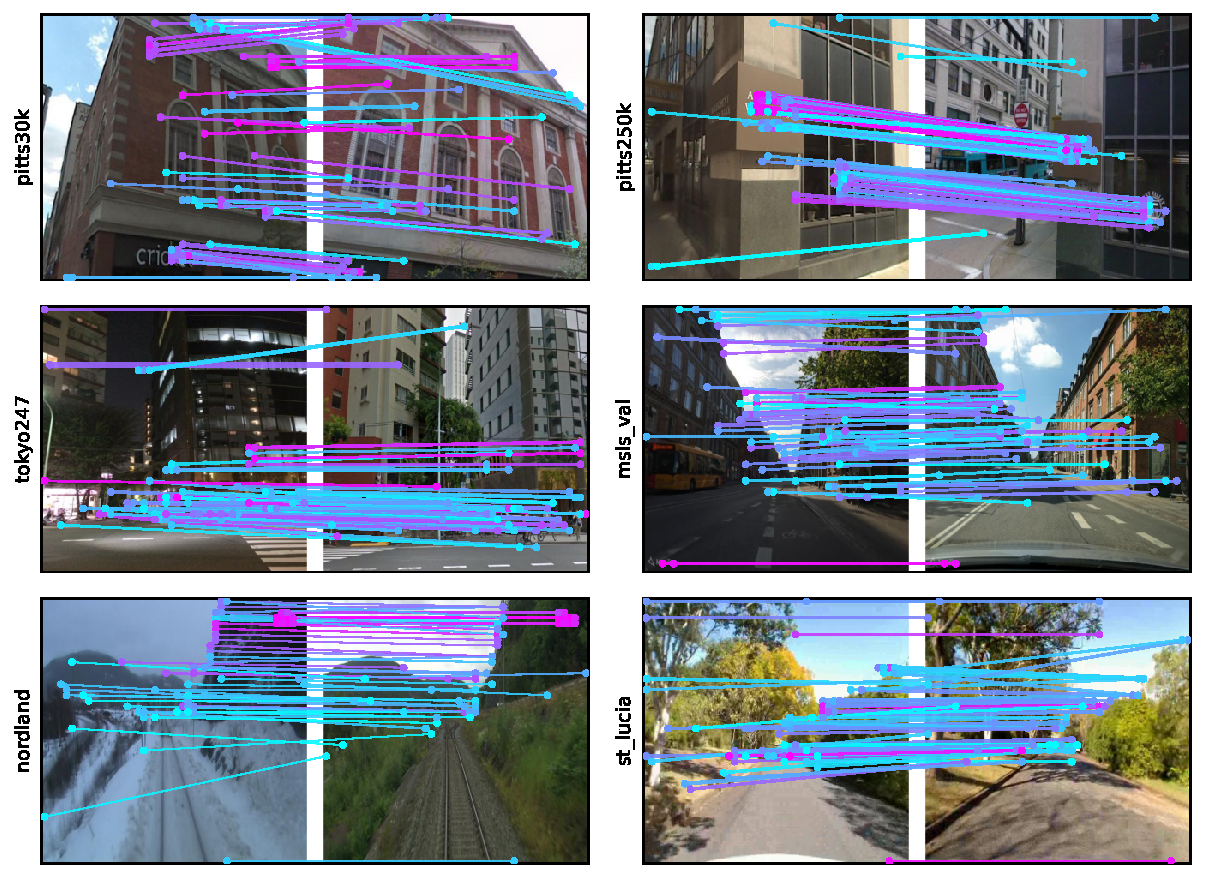
\includegraphics[width=\textwidth]{figures/all_maxsim_1.pdf}
\caption{\textsc{MaxSim} matches, benchmarks 1--6. Each line joins a query patch to its \textsc{MaxSim} partner in the retrieved image, drawn for the sixty largest contributions among the patches clearing the gate $\theta{=}0.65$ of \eqref{eq:stage2}; line colour is the row maximum $m_i$ and line width is that patch's contribution $c_i{=}w_i m_i$.}
\label{fig:vis-m1}
\end{figure*}
\begin{figure*}[p]
\centering
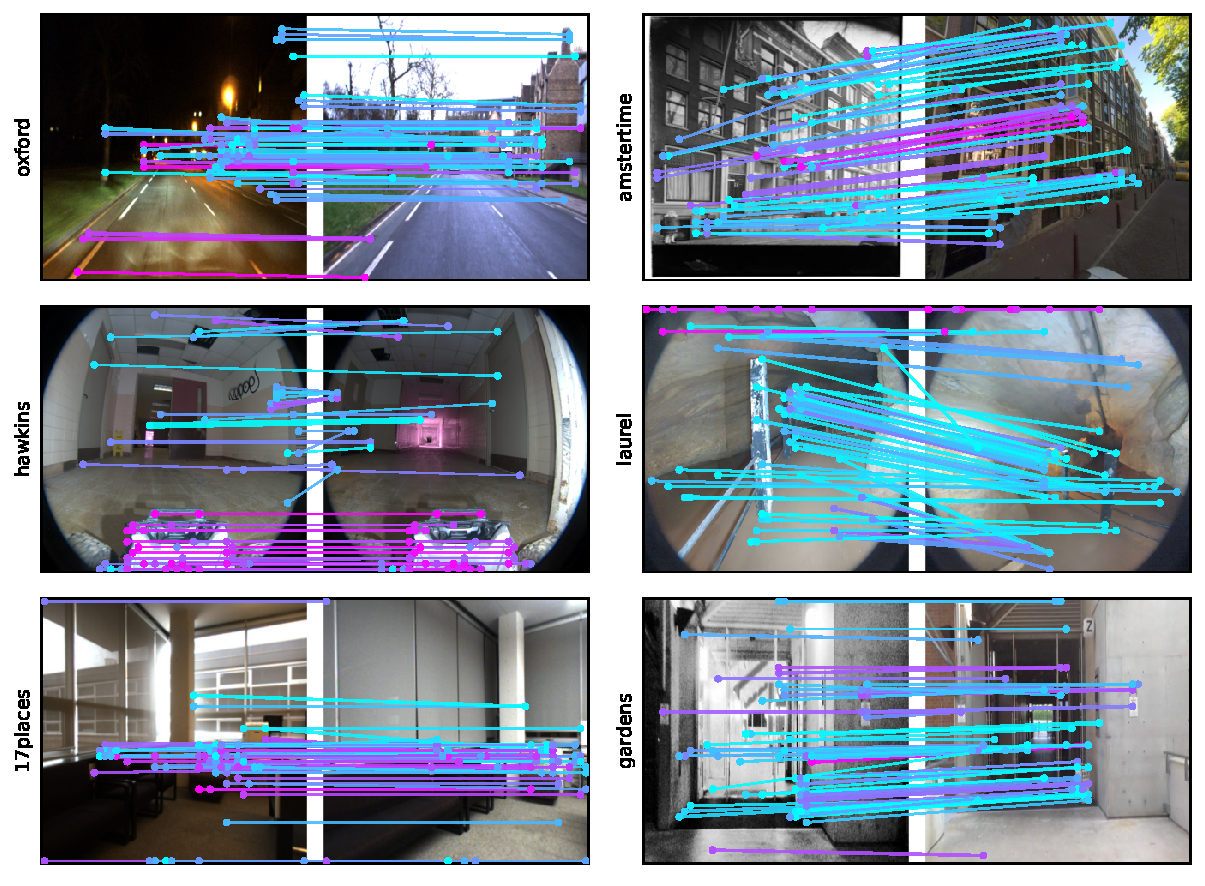
\includegraphics[width=\textwidth]{figures/all_maxsim_2.pdf}
\caption{\textsc{MaxSim} matches, benchmarks 7--12.}
\label{fig:vis-m2}
\end{figure*}
\begin{figure*}[p]
\centering
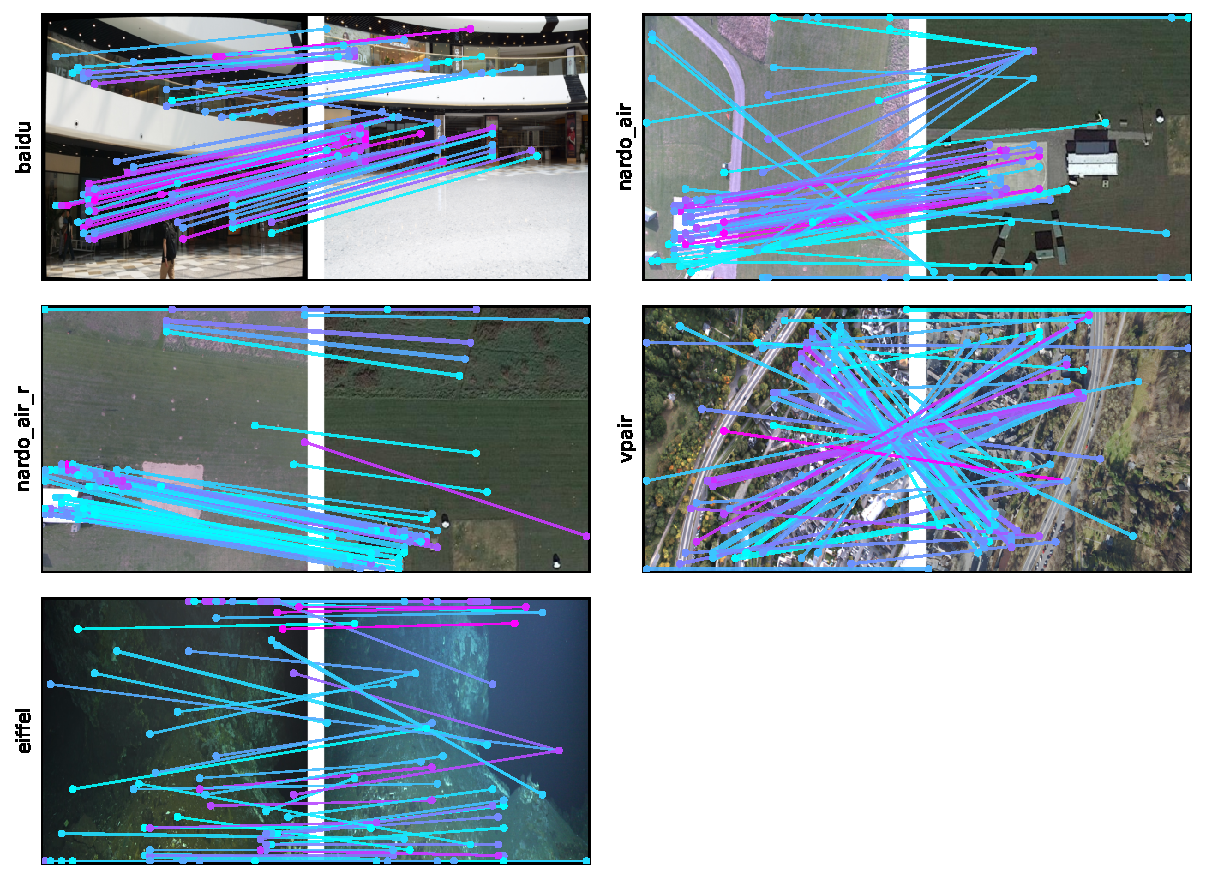
\includegraphics[width=\textwidth]{figures/all_maxsim_3.pdf}
\caption{\textsc{MaxSim} matches, benchmarks 13--17.}
\label{fig:vis-m3}
\end{figure*}

\section{Protocols and constants}

\subsection{Evaluation protocol}
\label{app:protocol}
\begin{table}[t]
\caption{\textbf{Evaluation protocol, per benchmark.} Every method here---ours and every baseline---is run through this protocol: same splits, ground truth and database. We do not quote each paper's own number, since those use different ground-truth radii and query subsets.}
\label{tab:protocol}
\begin{center}
{\scriptsize\setlength{\tabcolsep}{3.2pt}%
\resizebox{\textwidth}{!}{%
\begin{tabular}{lrrrll}
\toprule
Dataset & Database & Queries & Positives & Ground truth & Notes \\
\midrule
\multicolumn{6}{l}{\emph{Urban / standard benchmarks}} \\
\midrule
Pitts30k & 10{,}000 & 6{,}816 & 142.1 & UTM $\le 25$\,m & NetVLAD's official pitts30k\_test.mat split \\
Pitts250k & 83{,}952 & 8{,}280 & 153.6 & UTM $\le 25$\,m & same convention, different .mat \\
Tokyo 24/7 & 75{,}984 & 315 & 118.3 & filename UTM $\le 25$\,m & the official \textbf{315} subset, not the 1125 one \\
MSLS-val & 18{,}871 & 740 & 10.8 & filename UTM $\le 25$\,m, distance only (no heading) & the \textbf{740} subset of \citet{patchnetvlad}; \citet{effovpr} report the 11k variant \\
Nordland & 27{,}592 & 27{,}592 & 21.0 & $\pm 10$ frames (\textbf{lenient}) & papers using $\pm 1$ frame report markedly lower numbers \\
St Lucia & 1{,}549 & 1{,}464 & 14.9 & filename UTM $\le 25$\,m & gmberton format \\
Oxford RobotCar & 191 & 191 & 14.2 & the .mat's own posDistThr $=16$\,m & the small vehicular split used by \citet{anyloc} \\
AmsterTime & 1{,}231 & 1{,}231 & 1.0 & old\_X$\leftrightarrow$new\_X, one positive & historical against present-day photographs \\
\midrule
\multicolumn{6}{l}{\emph{SF-XL (one imagery set: a design split and four test splits)}} \\
\midrule
SF-XL val$^\ast$ & 8{,}015 & 7{,}983 & 9.3 & UTM $\le 25$\,m & \textbf{design split}; appears in no main table \\
SF-XL test v1 & 2{,}805{,}840 & 1{,}000 & 124.2 & UTM $\le 25$\,m & the four test splits share one $2.8$M database \\
SF-XL test v2 & 2{,}805{,}840 & 598 & 188.3 & UTM $\le 25$\,m & not yet re-run for the baselines (\S\ref{sec:setup}) \\
SF-XL test night & 2{,}805{,}840 & 466 & 114.1 & UTM $\le 25$\,m &  \\
SF-XL test occl. & 2{,}805{,}840 & 76 & 151.9 & UTM $\le 25$\,m & $74$ queries have a positive \\
\midrule
\multicolumn{6}{l}{\emph{Beyond street view (AnyLoc suite)}} \\
\midrule
VP-Air \emph{(aerial)} & 12{,}706 & 2{,}706 & 7.0 & provided correspondences & AnyLoc convention: database $=$ references $+$ $10{,}000$ distractors \\
Nardo-Air \emph{(aerial)} & 102 & 71 & 6.1 & gt\_matches.csv, distance $\le 60$\,m &  \\
Nardo-Air R \emph{(aerial)} & 102 & 71 & 6.1 & as above & reference images rotated $90^\circ$ \\
Hawkins \emph{(subterranean)} & 127 & 118 & 10.6 & 2-D pose $\le 8$\,m & long corridor \\
Laurel Caverns \emph{(subterranean)} & 141 & 112 & 23.8 & 2-D pose $\le 8$\,m &  \\
17 Places \emph{(indoor)} & 406 & 406 & 10.9 & official ground\_truth\_new.npy &  \\
Baidu Mall \emph{(indoor)} & 689 & 2{,}292 & 35.1 & 2-D camera pose $\le 10$\,m & $2{,}248$ queries have a positive \\
Gardens Point \emph{(day/night)} & 200 & 200 & 5.0 & official gardens\_gt.npy & database $=$ day-right, queries $=$ night-right \\
Mid-Atlantic Ridge \emph{(underwater)} & 65 & 101 & 3.0 & eiffel\_gt[101:] & the Eiffel Tower deep-sea site \citep{eiffeltower}, which \citet{anyloc} files under the ridge it sits on \\
\bottomrule
\end{tabular}%
}%
}
\end{center}

\par\smallskip{\scriptsize\emph{Notes.} Each baseline runs at its own default input resolution. Three conventions on which published numbers split: Nordland uses the lenient $\pm10$-frame ground truth, Tokyo the $315$-query and MSLS the $740$-query subsets, and VP-Air's database carries AnyLoc's $10{,}000$ distractors. Re-ranking uses a pool of $P=\min(1000,|\mathcal{D}|)$ throughout. $^{\ast}$SF-XL val is the design split and appears in no results table.}
\end{table}



\end{document}
